\chapter{PROCESSAMENTO DE LINGUAGEM NATURAL}
\label{chp:pln}

Este capítulo apresenta uma revisão da literatura da área de \glsdesc{pln} iniciando com as principais aplicações e desafios (Seção \ref{sec:pln-aplicacoes-desafios}), seguido por métodos de avaliação (\ref{sec:pln-metodos-avaliacao}), pelos modelos matemáticos-computacionais (\ref{sec:pln-modelos-matematico-computacionais}), uma introdução a aprendizado em conjunto (\ref{sec:pln-aprendizado-conjunto}), \textit{tokenizadores} de subpalavras (\ref{sec:pln-tokenizer}), redes neurais artificiais (\ref{sec:pln-redes-neurais-artificiais}), e por fim uma discussão sobre o tema (\ref{sec:pln-discussion}).

\section{APLICAÇÕES E DESAFIOS}
\label{sec:pln-aplicacoes-desafios}

% [TODO] As aplicações e desafios parecem não relacionados a um tipo específico aplicação final, mas sim tarefas diretas da linguagem (verbo? paráfrase? negação?). OU seja, falta alguma coisa para indicar tarefas mais complexas.

% Fonte de pesquisa: quais são os tipos de problemas?
\textcite{Russell2009Artificial} agruparam as tarefas de \gls{pln} em classificação de texto, recuperação da informação e extração da informação. A classificação de textos propõe decidir qual conjunto pré-definido de classes um dado texto pertence. A recuperação da informação é a tarefa que busca encontrar documentos que são relevantes à necessidade de informação do usuário. A extração da informação é a tarefa de identificar ocorrências de uma classe particular de objetos e o relacionamento entre esses objetos.

\textcite{Bakarov2018SurveyWordEmbeddings} apresentou uma lista não exaustiva de tipos de problemas utilizados para avaliar a representação de palavras. Essa lista foi utilizada nessa revisão bibliográfica como base da pesquisa dos tipos de problemas no campo de \gls{pln} e o relacionamento com os três principais grupos de tarefas agrupados por \textcite{Russell2009Artificial} foram apresentados.

% Noun Phrase Chunking / Text Chunking / Shallow Parsing / Parse Tree Level 0 Construction
O problema de separação de textos em blocos consiste na divisão do texto em blocos de modo que palavras sintaticamente relacionadas sejam classificadas na mesma categoria. Os blocos podem ser, por exemplo, frases substantivas (NP) ou verbais (VP). Os blocos não possuem sobreposição, ou seja, uma dada palavra não pode fazer parte de mais de um bloco. Essa tarefa é útil na etapa de pré-processamento de textos para análise e é uma subtarefa do grupo de extração da informação \cite{Tjong2000Chunking}. 

% Named Entity Recognition / Reconhecimento de entidades relacionadas
O reconhecimento de entidades relacionadas é uma subtarefa do grupo de extração da informação com objetivo de classificar elementos de uma sentença em categorias pré-definidas como pessoas, localização, datas e outras classes. Sistemas mais especializados se concentram em uma gama limitada de entidades dado um domínio de interesse. Essas entidades são marcadas e podem ser utilizadas como um dos primeiros passos para a análise semântica de textos, sendo uma subtarefa para sistemas de gerenciamento de documentos, mineração de textos entre outros \cites{Collobert2011Natural}{Carvalho2012ReconhecimentoDE}.

% Sentiment Analysis / Análise de sentimentos / polaridade
Análise de sentimento é um caso particular do problema de classificação de textos. Ocorre quando um fragmento de texto precisa ser marcado de forma binária, representando uma polaridade positiva ou negativa. Trabalhos nessa área compreendem a identificação de sentimentos de palavras, sentenças, frases e documentos. Estudos mostraram que a classificação de intensidade de sentimento em níveis mais granulares, como frases, é importante para tarefas práticas de pergunta e resposta \cites{Yessenalina2011CompositionalMatrix}{Bakarov2018SurveyWordEmbeddings}.

% Semantic Role Labeling / Anotador de papeis semânticos / classificação de assuntos
O anotador de papeis semânticos, subtarefa da classificação de textos, busca recuperar a estrutura argumento-predicado de uma sentença com a proposta principal de determinar \enquote{quem fez o que para quem}, \enquote{quando} e \enquote{onde}. Dessa forma, pretende-se identificar as relações semânticas existentes entre o predicado, seus participantes e suas propriedades através de uma lista pré-definida de possíveis papéis semânticos \cites{He2017DeepSemantic}{Carvalho2012ReconhecimentoDE}.

% Negation scope / identificação de enegação de escopo
A identificação de negação de escopo pode ser considerada como uma tarefa do grupo de classificação de texto. Consiste em identificar se uma dada ação em uma determinada sentença é uma negação ou não. Negações podem aparecer de diversas formas, invertendo não somente o significado de uma palavra, mas também de uma sentença completa. Negações também podem inverter o sentido de sentenças de forma implícita \cites{Ettinger2016ProbingForSemantic}{Prollochs2016NegationScopeDetection}.

% Part-of-Speech Tagging / detecção de idioma
A etiquetagem morfossintática, podendo ser classificado como extração e recuperação da informação, é uma tarefa que consiste em etiquetar palavras, expressões multipalavras e sinais de pontuação de uma sentença conforme suas categorias gramaticais, por exemplo, substantivos, verbos, adjetivos, etc. Essa tarefa é requerida por outras aplicações do \gls{pln}, tais como análise gramatical, tradução automática e por aplicações de processamento de fala, como por exemplo síntese de fala \cite{Domingues2011Abordagem}.

% Metaphor Detection and Paraphrase Detection  / detecção de metáfora / duplicate detection/ paraphrase identification/ record linkage / approximate string matching / text- to-text similarity detection
Outras tarefas relacionadas ao \gls{pln} são as metáforas e paráfrases. Segundo \textcite{Gao2018NeuralMetaphoDetection}, a detecção de metáforas pode se dividir em tarefas de classificação de textos, onde busca-se a classificação de um verbo em uma sentença como metafórico ou não; ou extração da informação, quando o desafio for indicar todas as palavras metafóricas independente de sua classificação morfossintática.

Conforme \textcite{Polastri2016Aprendizado}, a detecção de paráfrases e seu reconhecimento pode ser utilizada, por exemplo, na tradução automática, em que paráfrases podem ser empregadas para aumentar a cobertura estatística; na sumarização de multidocumentos, em que a identificação de paráfrases permite o reconhecimento de informações repetidas; e na geração de língua natural, em que as paráfrases permitem uma maior fluidez.

% Talvez adicionar recomendação palavras-chaves, recomendação da próxima palavra, recuperação de informação.

\section{MÉTODOS DE AVALIAÇÃO}
\label{sec:pln-metodos-avaliacao}

% [TODO] Parece muito focado em word embeddings, talvez devesse ser uma sub Seção dele.

Segundo \textcite{Bakarov2018SurveyWordEmbeddings}, os métodos de avaliação de desempenho de modelos de vetorização de palavras em \gls{pln} podem ser categorizados em intrínsecos e extrínsecos. Tais métodos podem ser utilizados como substrato ao entendimento das necessidades específicas de avaliações de outros modelos de \gls{pln}.

Os métodos de avaliação extrínsecos são baseados na habilidade dos modelos serem utilizados como vetores de características em algoritmos de aprendizado de máquina supervisionados em diversas aplicações de \gls{pln}. O desempenho do modelo supervisionado é então utilizado como métrica da tarefa específica, seja ela classificação, recuperação, extração de informação ou outra. Alguns pesquisadores afirmam que a vetorização com bom desempenho em uma aplicação, também terá um bom desempenho em outras tarefas, portanto, os resultados dos modelos em diferentes tarefas se correlacionam. Desse modo, os próprios resultados finais das aplicações podem ser utilizados como métricas de desempenho da modelagem vetorial de palavras.

Os métodos de avaliação intrínsecos são experimentos em que modelos são comparados com o julgamento humano sobre o relacionamento entre palavras. Conjuntos de palavras manualmente criados são usados frequentemente para obter avaliações humanas, e então essas avaliações são comparadas com o resultado produzido a partir da redução de dimensionalidade vetorial \cite{Bakarov2018SurveyWordEmbeddings}. Esses métodos baseiam-se nas pesquisas de semântica distribucional, as quais afirmam que existe uma similaridade semântica entre palavras, e palavras com maior relacionamento aparecem em contextos linguísticos semelhantes. \cite{Lenci2008Distributional}.

A seguir serão apresentadas medidas de relacionamento semântico. Tais medidas podem ser utilizadas como métricas de desempenho de representação vetorial em bases de dados supervisionados. Desse modo, os diferentes resultados dos relacionamentos semânticos de um modelo de representação vetorial podem ser comparados com tais bases de dados supervisionados e assim indicar o desempenho da representação vetorial.

% Cosine Similarity
Uma medida de relacionamento semântico em conjuntos de dados que utilizam representações vetoriais é o cosseno do ângulo entre dois vetores. Como observado por \textcite{Singhal2001Modern}, o cosseno possui uma propriedade que seu valor é igual a 1 quando os vetores forem iguais e 0 quando forem ortogonais. Desse modo, espera-se que sinônimos possuam valor próximo a 1. Alternativamente, o produto escalar entre dois vetores é geralmente utilizado como medida de similaridade. Se os vetores forem unários, o produto escalar é o próprio cosseno. A medida do cosseno entre vetores de palavras é conhecida como similaridade de cosseno e é apresentada na Equação \ref{eq:cosim} \cite{Orkphol2019WordSD}.
\begin{equation}
    \label{eq:cosim}
    cosseno(\vec{v_1}, \vec{v_2}) = \frac{\vec{v_1}.\vec{v_2}}{||\vec{v_1}||.||\vec{v_2}||}
\end{equation}

% Semantic Spaces and COsine Similarity / distâncias
A similaridade de cossenos também é utilizada como medida de similaridade em espaços semânticos de palavras. Conforme \textcite{Basile2014Enhanced}, espaços semânticos são espaços geométricos de palavras onde vetores expressam conceitos, e sua proximidade é uma medida de relacionamento semântico. Os conceitos são formados por composições de termos. Os termos são então combinados através da adição de vetores formando uma representação vetorial de uma sequência de termos de frases ou sentenças.

% Entropia / Maximum entropy / % cross-entropy para classificação de assuntos
Uma outra possibilidade, é a utilização da entropia. Em teoria da informação, a entropia é definida como uma forma de medida de incerteza de uma variável aleatória a respeito de fontes de informação. Assim, a entropia mede a quantidade de informação de uma variável aleatória. A entropia é máxima quando uma dada distribuição $p$ é uma distribuição uniforme e zero quando não há incerteza. A Equação \ref{eq:entropia} define a entropia de uma variável aleatória $V$ com valores $(v_1, \dots, v_K)$, cada qual com probabilidade $P(v_k)$ \cite{Russell2009Artificial}. 
\begin{equation} \label{eq:entropia}
    H(V) = - \sum_{k=1}^{K} P(v_k) \log_2 P(v_k)
\end{equation}

A avaliação também pode ser realizada através de categorização de conceitos. Nesse modelo, busca-se dividir um conjunto de palavras em diferentes categorias de subconjuntos. Essa divisão é então comparada com divisões produzidas por humanos. Pode-se, portanto, utilizar uma técnica chamada de máxima entropia para agrupar conteúdos textuais semelhantes. Segundo \textcite{Nigam99UsingMaximum}, o princípio da máxima entropia propõe que, quando não há dados estatísticos suficientes sobre uma determinada distribuição probabilística, que seja a distribuição considerada a mais uniforme possível. Desse modo, a máxima entropia pode ser utilizada para estimar qualquer distribuição probabilística.

Segundo \textcite{Goodfellow2016DeepLearning}, é possível medir o grau de diferença entre duas distribuições de probabilidades $P(x)$ e $Q(x)$ de uma mesma variável aleatória $x$ usando a divergência de Kullback-Leibler, KL (também conhecida como entropia relativa), conforme Equação \ref{eq:entropia_relativa}. A divergência de Kullback-Leibler é uma medida não simétrica e não negativa:
\begin{equation}
    \label{eq:entropia_relativa}
    D_{KL}(P||Q) = \sum_{x} P(x) \log \frac{P(X)}{Q(x)}
\end{equation}
sendo que, uma baixa divergência indica que as distribuições de probabilidades são parecidas, e o contrário indica que as distribuições de probabilidades são diferentes.

Uma outra medida relacionada à divergência de KL é a entropia cruzada. Minimizar a entropia cruzada em respeito a $Q$ é o equivalente a minimizar a divergência KL. A entropia cruzada é definida na Equação \ref{eq:entropia_cruzada} \cite{Goodfellow2016DeepLearning}.
\begin{equation}
    \label{eq:entropia_cruzada}
    H(P, Q) = H(P) + D_{KL}(P||Q)
\end{equation}

%[TODO] - Métricas de avaliação para Sequencial

\section{MODELOS MATEMÁTICO-COMPUTACIONAIS}
\label{sec:pln-modelos-matematico-computacionais}

%wordembedding
De acordo com \textcite{Bengio2003ANeuralProbabilistic}, um problema fundamental que torna a modelagem de linguagem natural complexa é a sua dimensionalidade. Por exemplo, ao modelar uma distribuição de probabilidade conjunta de 10 palavras consecutivas em linguagem natural com um vocabulário $V$ de tamanho $100.000$, existem $100000^{10} -1 = 10^{50} -1$ potencias parâmetros livres. Essa é a principal motivação dos modelos estatísticos Bayesianos Ingênuos, que utilizam da hipótese de independência de probabilidade entre n-gramas de palavras. 

Segundo \textcite{EthayarajhEtal2019Understanding}, modelos de \textit{word embedding} produzem representações distribuídas de palavras em um espaço contínuo de baixa dimensão. Essa representação é vetorial e é capaz de preservar as similaridades sintáticas e semânticas existentes entre palavras. Isto é, geralmente realizado utilizando redes neurais que predizem as palavras de um contexto, ou o contexto de uma palavra.

Existem modelos que criam representações vetoriais de palavras, tais modelos estão descritos nas seções: \ref{sec:word-embedding-lsa}, \ref{sec:word-embedding-sg}, \ref{sec:word-embedding-glove} e \ref{sec:word-embedding-fasttext}.

%tf-idf
\subsection{\glsentrylong{tf-idf}}

O \glsxtrfull{tf-idf} é uma medida estatística de relevância de palavras de um documento em relação a uma coleção de documentos ou corpus \cite{Rajaraman2011Mining}. A medida pode ser dividida em duas partes, a frequência que o termo ocorre em um documento (\textit{tf}) e o inverso da frequência dos documentos que contém o termo (\textit{idf}). Para a pergunta \enquote{agricultura no Brasil}, documentos que mencionam \enquote{agricultura} terão o resultado da medição \textit{tf} elevado. A palavra \enquote{no}, que aparece provavelmente em vários documentos, independentemente do tema, possui o inverso da frequência dos documentos, \textit{idf}, baixo. Assim, o termo \enquote{no} possui baixa relevância em relação a palavra \enquote{agricultura} e a palavra \enquote{Brasil} (adaptado de \textcite{Russell2009Artificial}).

O termo frequência, \textit{tf}, pode ser cálculo como se segue. Dado uma coleção de $N$ documentos, e que $f_{ij}$ seja o número de ocorrências do termo $i$ em um documento $j$. Então, o termo frequência ${TF}_{ij}$ é:
\begin{equation}
    \label{eq:tf}
    {TF}_{ij} = \frac{f_{ij}}{\max_k f_{kj}}
\end{equation}
portanto o termo frequência do termo $i$ no documento $j$ é $f_{ij}$ normalizado através da divisão pelo número de ocorrências máximo de qualquer termo no mesmo documento. Desse modo, o termo de maior ocorrência no documento $j$ possui $TF$ igual a 1, e todos os outros termos são frações de suas frequências. Dado um termo $i$, que aparece em $n_i$ dos $N$ documentos de uma coleção, o inverso da frequência dos documento é $IDF_i = \log_2(N/n_i)$. Assim, a medida \textit{tf-idf} para um termo $i$ em um documento $j$ é definida como
${TF}_{ij} \cdot {IDF}_i$. Os termos com as maiores medidas de \textit{tf-idf} são geralmente os termos que melhor caracterizam um tópico de um documento \cite{Rajaraman2011Mining}.

\subsection{Análise Semântica Latente} \label{sec:word-embedding-lsa}

A \gls{lsa} é uma abordagem completamente estatística para extrair relações entre palavras através do contexto em que é usada. A \gls{lsa} consiste na criação da matriz de termo-documento e sua transformação, como por exemplo \textit{Tf-Idf}; seguida pela redução dimensional através da \gls{svd}; e finalmente o processamento de similaridades como documento-documento, termo-termo e termo-documento quando aplicada a recuperação de informação \cite{Dumais2004LatentSA}.

Considerando uma matriz retangular $t \times d$ de termos e documentos, aplica-se a decomposição de valores singulares:
\begin{equation}
    \label{eq:lsa_svd}
    X = T \cdot S \cdot D^T
\end{equation}
onde $T$ é uma matriz $t \times r$ com colunas ortonormais, $D$ é uma matriz $d \times r$ com colunas ortonormais, e $S$ é uma matriz diagonal $r \times r$ com entradas ordenadas de modo decrescente. As entradas da matriz $S$ são os valores singulares, e as matrizes $T$ e $D$ são os valores singulares da esquerda e da direita, correspondendo aos vetores de termos e documentos para aplicações de recuperação de informação. A \gls{lsa} usa uma representação matricial incompleta da \gls{svd}, mantendo apenas os $k$ maiores valores singulares e seus vetores associados:
\begin{equation}
    \label{eq:lsa_svd_reduced_dimension}
    X = T_k \cdot S_k \cdot D_k^T
\end{equation}
sendo essa uma aproximação de mínimos quadrados de $X$ com $k$ parâmetros, e é o que a \gls{lsa} utiliza para representar seu espaço semântico. As linhas de $T_k$ são os vetores dos termos no espaço da \gls{lsa} e as linhas de $D_k$ são os vetores dos documentos no espaço da \gls{lsa} \cite{Dumais2004LatentSA}.

\subsection{O Modelo de N-Gramas}
\label{sec:n-grama}

%ngramas
O modelo n-gramas atribui probabilidade a uma sequência de elementos, seja uma sentença, sequência de palavras, caracteres entre outras granularidades. É um modelo baseado em uma cadeia de \textit{Markov} onde a probabilidade de seleção de um dado elemento é condicionado a elementos imediatamente anteriores. Uma n-grama é uma sequência de $N$ elementos, por exemplo: uma bigrama é uma sequência de dois elementos, uma trigrama é uma sequência de três elementos e assim sucessivamente \cite{Jurafsky2009Speech}.

Segundo \textcite{Jurafsky2009Speech}, a utilização da cadeia de \textit{Markov} simplifica o cálculo da probabilidade condicional. Considerando uma sequência de palavras $w_1, w_2, \dots, w_{n-1}$ representada por $w_1^{n-1}$, temos a aproximação:
\begin{equation}
    \label{eq:n_gram_approximation}
    P(w_n|w_1^{n-1}) \approx P(w_n|w_{n-N+1}^{n-1})
\end{equation}
e considerando regra da cadeia de probabilidade:
\begin{equation}
    \label{eq:n_gram_chain_rule}
    P(w_1^n) = P(w_1) P(w_2|w_1) P(w_3|w_1^{2}) \dots P(w_n|w_1^{n-1}) = \prod_{k=1}^n P(w_k|w_1^{k-1})
\end{equation}
pode-se computar a probabilidade total de uma sequência de palavras de uma bigrama como:
\begin{equation}
    \label{eq:n_gram_bi_gram}
    P(w_1^n) \approx \prod_{k=1}^n P(w_k|w_{k-1})
\end{equation}

Para estimar a probabilidade de uma n-grama pode-se utilizar a máxima verossimilhança. Para isso, é necessário contar a quantidade de vezes que uma dada n-grama ocorre no corpus e normalizar pela soma de todas as n-gramas que compartilham as mesmas palavras predecessoras. Por exemplo, para uma bigrama temos:
\begin{equation}
    \label{eq:n_gram_bi_gram_probaility}
    P(w_n|w_{n-1}) = \frac{C(w_{n-1}w_n)}{\sum_w C(w_{n-1}w)} = \frac{C(w_{n-1}w_n)}{C(w_{n-1})}
\end{equation}
onde a função $C$ é a contagem em um dado corpus \cite{Jurafsky2009Speech}.

\subsection{O Modelo de \textit{Skip-Gram}}
\label{sec:word-embedding-sg}

% skip-gram model - word2vec
Segundo \textcite{Goldberg2014word2vecED}, o modelo \textit{Skip-Gram} tenta predizer as palavras do contexto de origem dado uma palavra alvo. O modelo \textit{Skip-Gram}, representado na Figura \ref{fig:skip-gram}, pode ser simplificado como uma rede neural com uma camada oculta $W$ e uma camada de saída $W^\prime$. Sua entrada é um vetor $V$, com tamanho igual ao vocabulário do corpus, em que, palavras do contexto possuem valor 1 e todas as outras valor 0.

\begin{figure}[htbp]
    \centering
        \caption{O modelo \textit{Skip-Gram}.}
        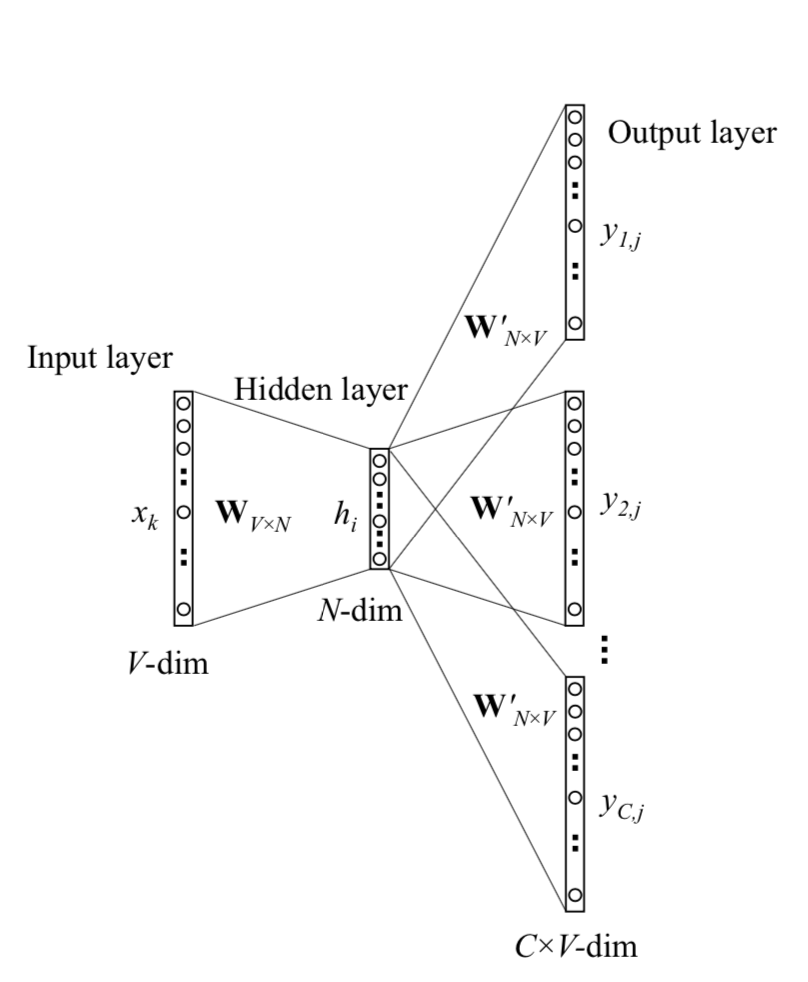
\includegraphics[scale=0.7]{resources/images/pln/skip-gram.png}
        \smallcaption{Fonte: \citefloat{Rong2014word2vec}, p. 6.}
        \label{fig:skip-gram}
\end{figure}

Formalmente, dado um corpus $T$ de palavras $w$, contexto $c$, de probabilidade condicional $p(c|w)$, o objetivo é parametrizar $\theta$ de $p(c|w;\theta)$ de modo a maximizar a probabilidade do corpus:
\begin{equation}
    \label{eq:skip_gram_full}
    \argmax_\theta \prod_{w \in T} \left [ \prod_{c \in C(w)} p({c}|{w};\theta) \right ]
\end{equation}
em que $c(w)$ é o conjunto de contextos da palavra $w$. Alternativamente:
\begin{equation}
    \label{eq:skip_gram}
    \argmax_\theta \prod_{(w,c) \in D} p({c}|{w};\theta)
\end{equation}
onde $D$ é o conjunto de todos os pares de palavras e contextos extraídos do corpus. A parametrização pode utilizar uma função exponencial normalizada (\textit{softmax}):
\begin{equation}
    \label{eq:skip_gram_p_c_dado_w}
    p(c|w;\theta) = \frac{e^{v_c v_w}}{\sum_{c^\prime \in C} e^{v_{c^\prime}.v_w}}
\end{equation}
em que $v_c$ e $v_w \in \mathbb{R}^d$ são representações vetoriais para $c$ e $w$ respectivamente e $C$ é o conjunto de todos os contextos. Os parâmetros $\theta$ são $v_{ci}$, $v_{wi}$ para $w \in V$, $c \in C$, $i \in 1 \dots d$; totalizando $|C| \times |V| \times |d|$ parâmetros. 

Aplicando a função logarítmica e utilizando soma ao invés de produto, temos:
\begin{equation}
    \label{eq:skip_gram_somatoria}
    \argmax_\theta \sum_{(w,c) \in D} \log p(c|w) = \sum_{(w,c) \in D} \left ( \log e^{v_c . v_w} - \log \sum_{c^\prime} e^{v_{c^\prime} . v_w} \right )
\end{equation}
e a maximização do objeto da Equação \ref{eq:skip_gram_somatoria} resultará em uma boa representatividade de $v_w \forall w \in V$, de modo que palavras similares possuirão vetores similares \cite{Goldberg2014word2vecED}.

% Softmax hieráquico
% [TODO] Parece que as simbologias do Mikolov são diferentes do Goldberg (Seção anterior). Alterar para uma simbologia consistentes
O \textit{softmax} hierárquico é uma aproximação computacionalmente eficiente do \textit{softmax}. O \textit{softmax} verifica $W$ nós de saída da rede neural para obter a distribuição de probabilidade, enquanto o \textit{softmax} hierárquico verifica aproximadamente $\log_2 (W)$ nós. Isso ocorre devido a versão hierárquica utilizar uma árvore binária representando a camada de saída onde as $W$ palavras são posicionadas nas folhas da árvore, e cada nó representa explicitamente a probabilidade relativa dos seus nós filhos \cite{Mikolov2013DistributedRepresentations}.

Formalmente, cada palavra $w$ pode ser alcançada por um caminho a partir do nó raiz da árvore. Sendo $n(w, j)$ o j-ésimo nó do caminho entre a raiz e a palavra $w$, e $L(w)$ o comprimento do caminho, então $n(w, 1) = raiz$ e $n(w, L(w)) = w$. Considerando também que para qualquer nó $n$ pertencente ao caminho, $ch(n)$ é um filho arbitrário qualquer do nó $n$ e $\llbracket x \rrbracket$ é 1 se $x$ é verdadeiro ou -1 caso contrário. Assim o \textit{softmax} hierárquico define $p(w_O|w_I)$ como:
\begin{equation}
    \label{eq:softmax_hierárquivo}
    p(w|w_I) = \prod_{j=1}^{L(w) - 1} \sigma \left ( \llbracket n(w, j + 1) = ch(n(w, j) \rrbracket . v_{n(w, j)}^{\prime T} v_{w_I} \right )
\end{equation}
em que $\sigma(x) = \frac{1}{1 + exp(-x)}$ e $\sum_{w=1}^{W} p(w|w_I) = 1$. Isso implica que o custo de computar $\log p(w_O|w_I)$  e $\nabla \log p (w_O|w_I)$ é proporcional a $L(w_O)$, o que em média não é maior do que $\log W$ \cite{Mikolov2013DistributedRepresentations}.

A estrutura da árvore utilizada pelo \textit{softmax} hierárquico possui efeito considerável na performance. Desse modo, \textcite{Mikolov2013DistributedRepresentations} utilizou uma árvore binária de \textit{Huffman} no modelo \textit{Skip-Gram} já que ela assinala códigos curtos para palavras frequente e resulta em um treinamento mais rápido.

% Amostragem negativa
Uma alternativa ao \textit{softmax} hierárquico é a amostragem negativa. Segundo \cite{Mikolov2013DistributedRepresentations}, um bom modelo deve ser capaz de diferenciar um dado verdadeiro de um ruído através da regressão logística. Considere $(w, c)$ o par palavra-contexto, e $p(D=1|w,c)$ a probabilidade de $(w,c)$ ser um dado verdadeiro, isto é, oriundo do corpus, e $p(D=0|w,c) = 1 - p(D=1|w,c)$ não ser oriundo do corpus, mas sim um ruído. Considere também que existem parâmetros $\theta$ controlando a distribuição $p(D=1|w,c;\theta)$. O objetivo é encontrar os parâmetros que maximizam a probabilidade que todas as observações sejam, de fato, dados verdadeiros:
\begin{equation}
    \label{eq:negative_sampling_expanded}
    \argmax_\theta \sum_{(w,c) \in D} \log p(D=1|w,c;\theta)
\end{equation}
a quantidade $p(D=1|c,w;\theta)$ pode ser definida utilizando \textit{softmax}:
\begin{equation}
    \label{eq:negative_sampling_softmax}
   p(D=1|w,c;\theta) = \frac{1}{1+exp(-v_c . v_w)}
\end{equation}
esse objetivo possui solução trivial se o $\theta$ for condicionado a $p(D=1|w,c;\theta)=1$ para cada par $(w,c)$. Desse modo, utiliza-se também um conjunto $D^\prime$ de pares $(w,c)$ aleatórios e assume que todos esses pares aleatórios são ruídos. O nome, amostragem negativa, se deve ao fato do conjunto $D^\prime$ ser um exemplo negativo. O objetivo da otimização é:
\begin{equation}
    \label{eq:negative_sampling_softmax_noise}
    \argmax_\theta \sum_{(w,c) \in D} \log \frac{1}{1+\exp(-v_c.v_w)} + \sum_{(e,c) \in D} \log \frac{1}{1+\exp(v_c . v_w)}
\end{equation}
considerando $\sigma(x) = \frac{1}{1+\exp(-x)}$:
\begin{equation}
    \label{eq:negative_sampling}
    \argmax_\theta \sum_{(w,c) \in D} \log \sigma(v_c .v_w) + \sum_{(e,c) \in D} \log \sigma(-v_c.v_w)
\end{equation}
\cite{Goldberg2014word2vecED}.

% Subamostragem de palavras frequentes
A presença de palavras frequentes em um corpus muito grande pode indicar que essas palavras possuem menos informações do que palavras raras. Por exemplo, uma grande quantidade de palavras pode    ocorrer no mesmo contexto que a palavra \enquote{em}, sendo que o modelo \textit{Skip-Gram} não se beneficia com esse relacionamento, mas sim com observações probabilísticas entre \enquote{Brasil} e \enquote{São Paulo}, por exemplo. Com a finalidade de balancear as palavras frequentes de palavras raras, um método de subamostragem é utilizado. Cada palavra $w_i$ do conjunto de treinamento é descartada utilizando a equação:
\begin{equation}
    \label{eq:skip_gram_sub_sampling}
    P(w_i) = 1 - \sqrt{\frac{t}{f(w_i)}}
\end{equation}
onde $f(w_i)$ é a frequência da palavra $w_i$ e $t$ é o limiar escolhido. \cite{Mikolov2013DistributedRepresentations}.

Foi demonstrado por \textcite{Mikolov2013DistributedRepresentations}, que a amostragem negativa possui maior precisão semântica e sintática do que o \textit{softmax} hierárquico utilizando árvore binária de \textit{Huffman}. 

Segundo \textcite{Gouws2016TrainingNeuralWE}, devido a simplicidade do modelo e a eficiência do algoritmo de treinamento, foi possível escalar o conjunto de dados de treinamento para mais de um bilhão de palavras com um vocabulário próximo a 700 mil palavras, e treinar o modelo em poucas horas em um computador desktop.

\subsection{GloVe}
\label{sec:word-embedding-glove}

De acordo com \textcite{Pennington2014GloveGV}, podemos agrupar os métodos de aprendizado de vetores de palavras em duas famílias, sendo: os métodos baseados em fatoração de matrizes, como a \gls{lsa}, e os métodos de janela de contexto local, como o \textit{Skip-Gram}. Os métodos como o \gls{lsa} utilizam informações estatística eficientemente, porém seus vetores possuem um desempenho ruim em tarefas de similaridade semântica e sintática. Por outro lado, os métodos como o \textit{Skip-Gram} possuem um desempenho superior em tarefas de similaridade semântica e sintática, porém não utilizam eficientemente as estatísticas do corpus, já que o contexto é dividido em janelas locais ao invés da utilização de contadores globais de coocorrência.

O modelo GloVe propõe a utilização das estatísticas de ocorrência das palavras em corpus como fonte principal para o aprendizado de representações vetoriais, com a capacidade de representar similaridades semânticas e sintáticas. 

Considere $X$ uma matriz de coocorrências de frequência de palavras, onde $X_{ij}$ representa o número de vezes que a palavra $j$ ocorre no contexto da palavra $i$ e que $X_i = \sum_k X_{ik}$ é o número de vezes que qualquer palavra ocorre no contexto da palavra $X_i$. Considere também $P_{ij} = P(j|i) = X_{ij}/X_i$ a probabilidade da palavra $j$ aparecer no contexto da palavra $i$.

Segundo \textcite{Pennington2014GloveGV}, a razão das probabilidades de coocorrências possui uma significância maior do que as próprias probabilidades. Quando a razão das probabilidades condicionais for próxima a 1, significa que ambas palavras possuem a mesma relevância no contexto da palavra alvo. Quando a razão for distante de 1, uma palavra possui maior relevância do que outra. A Tabela \ref{table:glove_prob_coocorrencia} apresenta as probabilidades e suas razões de um exemplo concreto. É possível notar que algumas palavras (\textit{solid} e \textit{gas}) são mais relevantes do que outras palavras (\textit{water} e \textit{fashion}) pois as razões são distantes do valor unitário. 

\begin{table}[ht!]
    \caption[Probabilidade de coocorrências de palavras]{Probabilidades de coocorrências para palavras alvo \textit{ice} e \textit{steam} com contexto selecionado a partir de um corpus de seis bilhões de \textit{tokens}}
    \label{table:glove_prob_coocorrencia}
    \centering
    \begin{tabular}{c|c|c|c|c}
        \hline
        Probabilidade e Razão & k=solid         & k=gas           & k=water         & k=fashion       \\
        \hline
        $P(k|ice)$            & $1.9 \times 10^{-4}$ & $6.6 \times 10^{-5}$ & $3.0 \times 10^{-3}$ & $1.7 \times 10^{-5}$ \\
        \hline
        $P(k|steam)$          & $2.2 \times 10^{-5}$ & $7.8 \times 10^{-4}$ & $2.2 \times 10^{-3}$ & $1.8 \times 10^{-5}$ \\
        \hline
        $P(k|ice)/P(k|steam)$ & $8.9$           & $8.5 \times 10^{-2}$ & $1.36$          & $0.96$          \\
        \hline
    \end{tabular}
    \smallcaption{Fonte: \citefloat{Pennington2014GloveGV}}
\end{table}

Utilizando o conceito introduzido no parágrafo anterior, pode-se construir um ponto de partida para o aprendizado de vetores de palavras com base nas razões de probabilidades de coocorrência:
\begin{equation}
    \label{eq:glove_model_start_point}
    F(w_i, w_j, w^*_k) = \frac{P_{ik}}{P_{ij}}
\end{equation}
onde $w \in \mathbb{R}^d$ são vetores de palavras e $w^* \in \mathbb{R}^d$ são contextos de palavras diferentes de $w$. Para codificar a razão $P_{ik}/P_{jk}$ no espaço vetorial de palavras utiliza-se a relação linear de diferenças entre vetores:
\begin{equation}
    \label{eq:glove_model_linearity}
    F(w_i - w_j, w^*_k) = \frac{P_{ik}}{P_{ij}}
\end{equation}
nota-se que os argumentos de $F$ são vetores enquanto o lado direito da equação é um escalar. Com a finalidade de simplificar $F$, é realizado o produto escalar dos argumentos:
\begin{equation}
    \label{eq:glove_model_dot_product}
    F((w_i - w_j)^T w^*_k) = \frac{P_{ik}}{P_{ij}}
\end{equation}
em um contexto de matrizes de coocorrência entre palavras, a distinção entre uma palavra e seu contexto é arbitrário, portanto, operações de troca como $w \xleftrightarrow{} w^*$ e também $X \xleftrightarrow{} X^T$ devem ser permitidas. Como parte da solução, $F$ é definida como uma função exponencial e um modelo de regressão utilizando mínimos quadrados ponderados é utilizado:
\begin{equation}
    \label{eq:glove_model_least_square}
    J = \sum_{i,j=1}^{V} f(X_{ij}) \left ( w_i^T w^*_j + bi + b*_j - \log X_{ij} \right ) ^2
\end{equation}
onde $V$ é o tamanho do vocabulário, $b_i$ é o viés de $wi$ e $b*_j$ é o viés de $w^*_k$. O termo $f(X_{ij})$ é utilizado como função de ponderação para evitar com que termos raros e com pouca importância em relação aos termos mais frequentes causem ruído. A função $f$ é definida por:
\begin{equation}
    \label{eq:glove_model_weight}
    f(x)= 
    \begin{cases}
        (x/x_{max})^\alpha,& \text{se } x < x_{max} \\
        1,                 & \text{caso contrário}
    \end{cases}
\end{equation}
em que $\alpha = 3/4$.

\subsection{FastText}
\label{sec:word-embedding-fasttext}

Segundo \textcite{Bojanowski2016Bojanowski}, ambos modelos, Word2Vec, representado no presente trabalho pelo \textit{Skip-Gram} e GloVe, representam cada palavra do vocabulário como vetores distintos, sem compartilhar parâmetros, ignorando a estrutura interna das palavras. Idiomas como o Francês e o Espanhol possuem mais de 40 formas diferentes de flexões verbais para a maioria do verbos, e a língua Finlandesa possui mais de 15 casos para substantivos. Esses idiomas possuem muitas formas de palavras que raramente ocorrem no corpus de treinamento, podendo até não ocorrer nenhuma vez, fazendo com que seja difícil aprender boas representações de palavras.

O modelo FastText aprende representações a partir de n-gramas de caracteres e representa as palavras como a soma dos vetores de n-gramas. Esse modelo considera informações morfológicas das palavras, ele é considerado uma extensão do modelo \textit{Skip-Gram}.

% cesta de caracteres - bag of character
Cada palavra $w$ é representada como uma cesta de n-gramas de caracteres. Os símbolos \textit{<} e \textit{>} são adicionados no início e no fim das palavras, o que permite a distinção de prefixos e sufixos de outras sequências de caracteres. Adicionalmente, a palavra $w$ é adicionada ao seu próprio conjunto de n-gramas. Utilizando a palavra \enquote{coisa} e $n = 3$ como exemplo, a cesta de n-gramas é representada por: \textit{<co}, \textit{coi}, \textit{ois}, \textit{isa}, \textit{sa>}, e a sequência especial é \textit{<coisa>} \cite{Bojanowski2016Bojanowski}.

Considerando um dicionário de n-gramas de tamanho $G$ e dado uma palavra $w$, a representação $G_w \subset \{1,\dots,G\}$ denota o conjunto de n-gramas que ocorrem em $w$. A representação vetorial $z_g$ é associada a cada n-grama $g$. Uma palavra é representada pela soma de todas as representações vetoriais de suas n-gramas. A função de avaliação é definida como:
\begin{equation}
    \label{eq:fasttext_model_score}
    s(w, c) = \sum_{g \in G_w} z_g^T v_c 
\end{equation}
Esse modelo permite compartilhar representações entre palavras, tornando o aprendizado de palavras raras confiável \cite{Bojanowski2016Bojanowski}.

\section{APRENDIZADO EM CONJUNTO}
\label{sec:pln-aprendizado-conjunto}

% Ensemble Learning
\textcite{Yin2015LearningWM} experimentou alguns métodos de conjunção de aprendizado como: $CONC$, $SVD$, $1TON$ and $1TON+$. O método $CONC$, abreviação de concatenação, possui o \textit{meta-embedding} $w$ como a concatenação ponderada de $N$ outros conjuntos de representação normalizados sendo a ponderação um hiperparâmetro.

\textcite{ElBoukkouriEtal2019Embedding} classificou os métodos de \textit{word embeddings} em estáticos e contextualizados dependendo da dinâmica de representação vetorial realizada por eles. Os métodos estáticos atribuem a cada símbolo uma única representação independentemente do contexto que está inserido, como por exemplo o Word2Vec (Seção \ref{sec:word-embedding-sg}), GloVe (\ref{sec:word-embedding-glove} e FastText (\ref{sec:word-embedding-fasttext}). Por outro lado, os métodos dinâmicos produzem uma representação vetorial distinta para cada contexto como, por exemplo, o ELMo. Os modelos contextualizados usualmente possuem um melhor desempenho, porém necessitam de grandes quantidades de dados para serem treinados, o que pode ser uma dificuldade em domínios especializados.

Eles propuseram a combinação dos métodos estáticos treinados com corpora especializadas e dos modelos contextualizados utilizando uma simples concatenação de vetores ou uma somatória de vetores ponderada. Tal combinação resultou em um aumento de desempenho, independentemente do modelo estático escolhido, indicando a possibilidade de melhoria quando há pouco conteúdo disponível para um domínio especializado.

\section{\textit{TOKENIZADORES} DE SUBPALAVRAS}
\label{sec:pln-tokenizer}

Os \textit{tokenizadores} de subpalavras são um conjunto de métodos, inicialmente utilizados pelas \glspl{nmt}, para tratar o problema da existência de palavras raras. O vocabulário das redes neurais é usualmente limitado entre trinta e cinquenta mil palavras, porém, o \gls{pln} é considerado um problema de vocabulário aberto, especialmente em idiomas com processos produtivos de formação de palavras como aglutinação ou composição. Por exemplo, a palavra composta \textit{Abwasserbehandlungsanlage}, do idioma Alemão, significa \enquote{estação de tratamento de águas residuais}, indicando que uma representação segmentada e de tamanho variável é intuitivamente mais atraente do que uma codificação de palavras de tamanho fixo \cite{Sennrich2016Neural}.

Modelos a nível de palavras são incapazes de produzir resultados específicos, como uma tradução ou geração, de palavras não vistas durante o treinamento. Dessa forma, os \textit{tokenizadores} de subpalavras codificam palavras raras através de múltiplos níveis de granularidade, desde caracteres individuais até palavras completas, fazendo com que palavras raras sejam subdivididas em uma coleção de unidades de subpalavras, podendo atingir o nível mais elementar como uma sequencia de caracteres \cite{Bostrom2020BytePair}. A seguir serão apresentados os \textit{tokenizadores} \gls{bpe} (Seção \ref{sec:tokenizer-bpe}), WordPiece (\ref{sec:tokenizer-wordpiece}), \glsxtrfull{ml} uni-grama (\ref{sec:tokenizer-unigram}) e SentencePiece (\ref{sec:tokenizer-sentencepiece}).

\subsection{\glsentrylong{bpe}}
\label{sec:tokenizer-bpe}

O \glsxtrfull{bpe}, apresentado na sua forma de compressão de dados por \textcite{Gage1994ANewAlgorithm}, é um algoritmo que iterativamente substitui os pares de bytes mais utilizados em uma sequência por um único byte nunca utilizado antes. \textcite{Sennrich2016Neural} alteraram a substituição de pares de bytes para pares de palavras ou sequência de palavras, habilitando assim sua utilização em segmentadores de palavras.

Inicialmente é criado um vocabulário de caracteres e símbolos. Os pares de caracteres e símbolos são contados iterativamente e os mais frequentes são mesclados, por exemplo, se o par $(A, B)$ for o qual possui a maior contagem, ele será substituído por $(AB)$. Cada mescla produz um novo símbolo que pode representar uma n-grama de uma palavra (vide Seção \ref{sec:n-grama}), e eventualmente a palavra inteira. O tamanho final do vocabulário é igual ao tamanho inicial mais a quantidade de mesclas realizadas. Sua complexidade computacional é de $O(N \log(N))$ quando utilizado uma fila de prioridade (\textit{HEAP}). Seu pseudocódigo é apresentado na Figura \ref{alg:bpe-algorithm}.

\begin{algorithm}
    \caption{Pseudocódigo do \textit{tokenizador} \glsxtrlong{bpe}.}
    \Entrada{conjunto de \textit{strings} $D$, tamanho alvo do vocabulário $k$}
    \Saida{vocabulário $V$}
    $V \gets$ todos caracteres únicos de $D$\;
    \Enqto{$|V| < k$} {
        $t_E,t_D \gets$ bigrama mais frequente de $D$\;
        $t_{NOVO} \gets t_E + t_D$\;
        $V \gets V + [t_{NOVO}]$\;
        substitua cada ocorrência de $t_E,t_D$ em $D$ por $t_{NOVO}$\;
    }
    \Retorna{$V$}
    \smallcaption{Fonte: Autor \enquote{adaptado de} \citefloat{Sennrich2016Neural}, p. 4618.}
    \label{alg:bpe-algorithm}
\end{algorithm}

\subsection{WordPiece}
\label{sec:tokenizer-wordpiece}

O WordPiece, apresentado por \textcite{Schuster2012Japanese}, constrói o vocabulário de subpalavras de forma incremental, utilizando um algoritmo guloso, buscando aumentar a probabilidade máxima do \gls{ml} no corpus de treinamento. Os passos para isso são: (1) inicializar o inventário de subpalavras com os caracteres básico Unicode (2); construir um \gls{ml} usando o inventário da primeira etapa (3); gerar uma nova palavra, combinando duas palavras do inventário, de modo a aumentar a verossimilhança máxima do conjunto de treinamento (4); voltar para o segundo passo até atingir o tamanho desejado do vocabulário ou a verossimilhança ficar abaixo de um limiar. A Figura \ref{alg:wordpiece-algorithm} apresenta seu pseudocódigo.

\begin{algorithm}
    \caption{Pseudocódigo do \textit{tokenizador} de subpalavras WordPiece.}
    \Entrada{conjunto de \textit{strings} $D$, tamanho alvo do vocabulário $k$, verossimilhança mínima $z$}
    \Saida{vocabulário $V$}
    $V \gets$ todos os caracteres Unicode básicos incluindo todos os ASCII\;
    \Enqto{$|V| < k \And LL_{max} > z$} {
        $model \gets$ \gls{ml} de $D$ utilizando $V$\;
        $LL \gets []$\;
        \Para{todos pares de unidades $U_A,U_B \in V$} {
            $LL \gets LL + [$ \textit{verossimilhança}$(model + [U_A + U_B])]$\;
        }
        $LL_{max} \gets max(LL)$\;
        $U_E,U_D \gets$ par de unidades que gerou $LL_{max}$\;
        $U_{NEW} \gets U_E + U_D$\;
        $V \gets V + [U_{NEW}]$\;
    }
    \Retorna{$V$}
    \smallcaption{Fonte: Autor.}
    \label{alg:wordpiece-algorithm}
\end{algorithm}

O treinamento do segmentador de palavras é computacionalmente caro quando se verifica todos os pares de unidades disponíveis, isso ocorre porque um novo \gls{ml} deverá ser construído. Nesse caso, a complexidade computacional é de $O(K^2)$ por iteração, sendo que $K$ é o número de unidades de palavras de cada passo. Com a finalidade de otimizar o algoritmo, algumas heurísticas são utilizadas, por exemplo: (1) testar somente os pares que realmente existem no conjunto de treinamento; (2) testar somente os pares com chances elevadas de serem os melhores, e (3) combinação de múltiplos pares em uma única iteração \cite{Schuster2012Japanese}.

A abordagem do WordPiece é ligeiramente diferente do \textit{tokenizador} \gls{bpe} (Seção \ref{sec:tokenizer-bpe}). Ao invés de mesclar os bigramas mais frequentes, ele utiliza a verossimilhança máxima do \gls{ml} para decidir quais unidades serão mescladas.

\subsection{\glsentrylong{ml} Uni-grama}
\label{sec:tokenizer-unigram}

O \glsxtrfull{ml} uni-grama, também chamado de regularização subpalavra, proposto por \textcite{Kudo2018Subword}, foi motivado pela necessidade de tornar os \textit{tokenizadores} subpalavras determinísticos, em especial o \gls{bpe} (Seção \ref{sec:tokenizer-bpe}). Uma simples palavra como \enquote{olá} pode ser subdividida em três diferentes formas, \enquote{o+l+á}, \enquote{ol+á} e \enquote{o+lá} (o sinal $+$ indica a posição da divisão dos \textit{tokens}), sendo que, cada uma delas podem possuir vetores ou identificadores de unidade completamente diferentes.

O \gls{ml} uni-grama assume que cada subpalavra ocorre independentemente, e assim a probabilidade de uma sequência de subpalavras $X = (x_1, \dots, x_M)$ pode ser formulada como o produto das probabilidades de ocorrência de cada subpalavra $p(x_i)$:
\begin{equation}
\begin{aligned}
    \label{eq:unigram-model}
    & P(X) = \prod_{i=1}^{M} p(x_i)\\
    & \forall x_i \in V, \sum_{x \in V}p(x) = 1
\end{aligned}
\end{equation}
em que $V$ é um vocabulário pré-determinado. A segmentação mais provável $x^\star$ para a sentença de entrada $X$ é dada por:
\begin{equation}
    \label{eq:unigram-model-most-probable}
    x^\star = \argmax_{x \in S(X)} P(x)
\end{equation}
onde $S(X)$ é um conjunto de segmentações possíveis construídas a partir da sentença $X$ e $x^\star$ é obtido a partir do algoritmo de Viterbi.

Se o vocabulário $V$ for dado, isto é, o conjunto de todas as possíveis \textit{tokenizações}, as probabilidades de ocorrência de subpalavras $p(x_i)$ são estimadas através de algoritmos que maximizem a verossimilhança marginal $\mathcal{L}$ assumindo que $p(x_i)$ são variáveis escondidas:
\begin{equation}
    \label{eq:unigram-model-likelihood}
    \mathcal{L} = \sum_{i=1}^{|D|} log ( \sum_{x \in S(X^{(s)}} p(X))
\end{equation}
em que $D$ é o conjunto de strings do corpus. Seu pseudocódigo é apresentado na Figura \ref{alg:unigram-algorithm}.

\begin{algorithm}
    \caption{Pseudocódigo do \textit{tokenizador} de subpalavras utilizando \gls{ml} uni-grama.}
    \Entrada{conjunto de \textit{strings} $D$, tamanho alvo do vocabulário $k$}
    \Saida{vocabulário $V$}
    $V \gets$ todas as \textit{substrings} que ocorrem mais do que uma vez dentro de uma mesma palavra em $D$\;
    \Enqto{$|V| > k$} {
        Ajustar o \gls{ml} uni-grama $\phi$ para $D$\;
        \Para{$t \in D$}{
            $L_t \gets p_\phi(D) - p_{\phi\prime}(D)$\\
               onde $\phi\prime$ e o \gls{ml} sem o \textit{token} $t$\;
        }
        Remove $\min{|V| - k,\left \lfloor{\alpha|V|}\right \rfloor}$ dos \textit{tokens} $t$\\
        com maior $L_t$ de $V$, onde $\alpha in [0,1]$\\
        é um hiperparâmetro\;
    }
    Ajustar o \gls{ml} final do uni-grama $\phi$ para $D$
    \Retorna{$V$,$\phi$}
    \smallcaption{Fonte: Autor \enquote{adaptado de} \citefloat{Sennrich2016Neural}, p. 4618.}
    \label{alg:unigram-algorithm}
\end{algorithm}

\subsection{SentencePiece}
\label{sec:tokenizer-sentencepiece}

Em qualquer que seja a idioma, os \textit{tokenizadores} são normalmente seguidos por etapas de pré e pós-processamento, possuindo regras específicas para cada idioma. Por exemplo, os textos redigidos em idiomas Europeus são normalmente separados por espaços, porém tal afirmativa não é válida para textos em Japonês, Coreano ou Mandarim. \textcite{Kudo2018SentencePiece} propuseram um \textit{tokenizador} de textos agnóstico à linguagem utilizada através do emprego de algoritmos de segmentação em subpalavras.

O SentencePiece pode utilizar o \gls{bpe} e o \gls{ml} uni-grama como segmentadores de subpalavras, apresentados nas seções \ref{sec:tokenizer-bpe} e \ref{sec:tokenizer-unigram}, respectivamente, além da capacidade de treinar a partir do corpus sem alteração. Sua \textit{tokenização} é sem perdas, isto é, é possível reverter o processo de \textit{tokenização} conforme Equação \ref{eq:sentencepiece-lossless}.

Para que isso seja possível, seu processo é dividido em quatro componentes, sendo eles, Normalização, Treinamento, Codificação e Decodificação. A Normalização transforma caracteres Unicode semanticamente equivalentes em sua forma canônica. O segundo componente, Treinamento, treina o modelo de segmentação de subpalavra utilizando o texto normalizado. A Codificação, representando o \textit{tokenizador}, executa internamente o primeiro componente (Normalização) e \textit{tokeniza} ele em uma sequência de subpalavras utilizando o modelo do segundo componente (Treinamento). A Decodificação, representando o processo inverso da Codificação, converte uma sequência de subpalavras em um texto normalizado.
\begin{equation}
    \label{eq:sentencepiece-lossless}
    \textit{Decodificação}(\textit{Codificação}(\textit{Normalização}(\textit{texto}))) = \textit{Normalização}(\textit{texto})
\end{equation}

O modelo gerado pelo SentencePiece é autocontido, ele provê um arquivo de configuração que possui o vocabulário, parâmetros da segmentação e também o transdutor de estado finito utilizado para a normalização, sem a necessidade de qualquer tipo de dependência externa.

\section{REDES NEURAIS ARTIFICIAS}
\label{sec:pln-redes-neurais-artificiais}

A seguir, são apresentadas algumas topologias de redes neurais artificiais que esse trabalho teve grande influência. A Seção \ref{sec:rnn} apresenta o conceito de \glsxtrfull{rnn}, seu fundamento é utilizado para desenvolver as seções \ref{sec:lstm} e \ref{sec:gru} como especializações dessa topologia. A Seção \ref{sec:encoder-decoder}, demonstrando o conceito fundamental das \glsxtrfullpl{nmt}, e na Seção \ref{sec:encoder-decoder-attention} é apresentado o modelo de atenção, base para a elaboração da arquitetura \textit{Transformer}, apresentada na Seção \ref{sec:transformer}.

\subsection{\glsentrylong{rnn}}
\label{sec:rnn}

\glsxtrfullpl{rnn} são uma família de redes neurais específicas para processamento de dado sequencial. Esse tipo de rede compartilha seus parâmetros em diferentes partes do modelo, permitindo sua aplicação em condições não visitadas durante o treinamento, como sentenças de diferentes tamanhos. Elas fornecem uma saída com base na atualização das saídas anteriores \cite{Goodfellow2016DeepLearning}.

\textcite{Goodfellow2016DeepLearning} apresentaram a formulação da \gls{rnn} com base na forma clássica de sistema dinâmicos, isto é, na forma $s^{(t)} = f(s^{t-1}; \theta)$ em que $s{(t)}$ é o estado do sistema. Essa equação é recorrente porque o estado $s$ no tempo $t$ possui como referência o estado no tempo $t-1$. Sua forma desenrolada (do termo em inglês \textit{unfolded}) para o instante $\tau = 3$ é então $s^{(3)} = f(f(s^{(1)}; \theta); \theta)$, onde $s^{(1)}$ é o estado inicial. Desse modo, o processo de desenrolar pode ser entendido como a aplicação repetitiva de sua função até o estado inicial.

A Equação \ref{eq:rnn-base} considera um sistema com sinal externo $x^{(t)}$ e utiliza a variável $h$ para representar seu estado, a Figura \ref{fig:rnn-desenrolada} apresenta ambas as formas, enrolada e desenrolada, utilizando as variáveis $x$ e $h$.
\begin{equation}
    \label{eq:rnn-base}
    h^{(t)} = f(h^{(t-1)}, x^{(t)}; \theta)
\end{equation}

\begin{figure}[htbp]
    \centering
        \caption{\glsxtrlong{rnn} enrolada (esquerda) e desenrolada (direita).}
        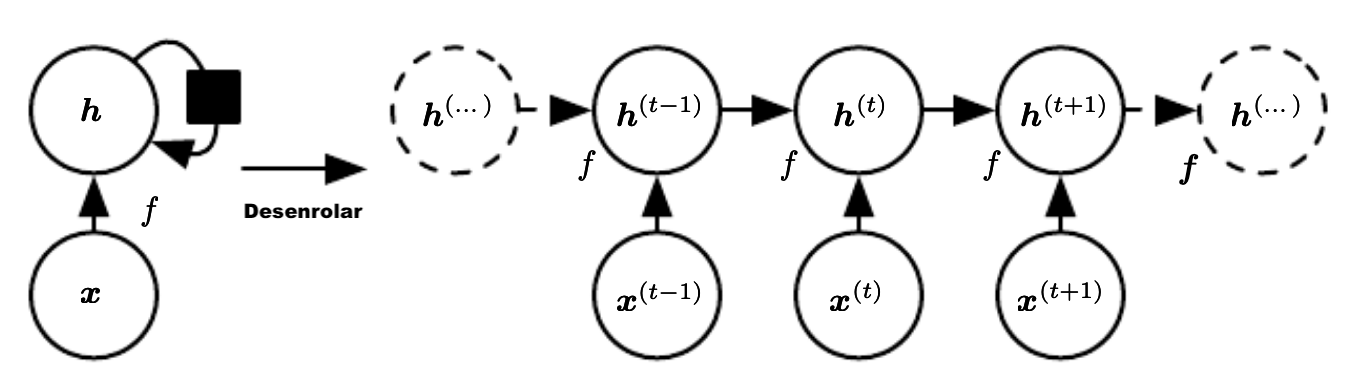
\includegraphics[scale=0.60]{resources/images/pln/rnn-desenrolada.png}
        \smallcaption{Fonte: Autor \enquote{adaptado de} \citefloat{Goodfellow2016DeepLearning}, p. 370.}
        \label{fig:rnn-desenrolada}
\end{figure}

Alguns padrões são comuns em redes recorrentes, como a produção de uma saída a cada passo e a recorrência ocorrendo através das unidades escondidas, ou a saída de um passo conectada a um estado escondido do próximo, ou até mesmo a produção de uma saída somente no último passo da recorrência. Uma rede recorrente, como no primeiro exemplo, ilustrada na Figura \ref{fig:rnn-turing}, pode processar qualquer função computável que uma máquina de \textit{Turing}, recebendo uma sequência binária como entrada, discretizando o resultado e assim, produzindo uma sequência binária de saída \cite{Goodfellow2016DeepLearning}.
\begin{figure}[htbp]
    \centering
        \caption[Detalhes da \glsxtrfull{rnn}.]{Detalhes da \glsxtrfull{rnn}. Grafo de uma rede recorrente que mapeia uma sequência de $x$ valores para uma sequência de $o$ valores. possui uma métrica $L$ que mede a distância de $o$ do alvo de treinamento $y$. A entrada $x$ é conectado a unidade escondida através de uma matriz de pesos $U$, e essas unidades são conectadas entre si por uma matriz de pesos $W$ e as saídas $o$ por uma matriz de pesos $V$.}
        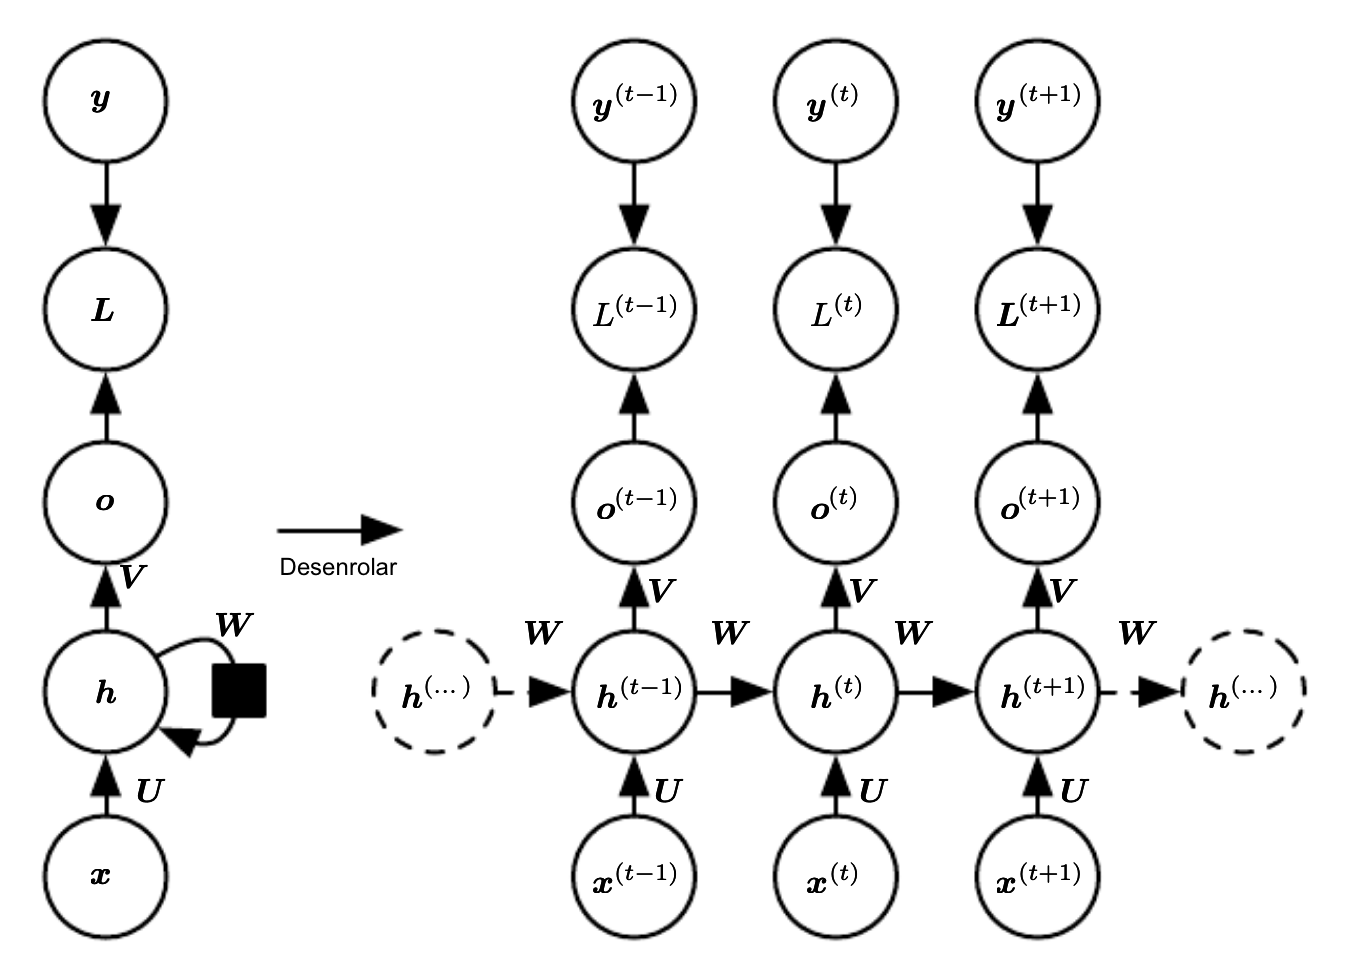
\includegraphics[scale=0.60]{resources/images/pln/rnn-turing.png}
        \smallcaption{Fonte: Autor \enquote{adaptado de} \citefloat{Goodfellow2016DeepLearning}, p. 373.}
        \label{fig:rnn-turing}
\end{figure}

A passagem direta, ou para frente (\textit{feedforward}), necessita de uma função de ativação na direção da unidade escondida para a saída. A saída pode ser discreta, como é o caso de predição de palavras ou caracteres. Nesse caso, uma forma natural de representação é através de uma probabilidade logarítmica para cada valor possível da variável discreta, sendo então possível gerar um vetor $\hat{y}$ de probabilidades normalizadas.

As equações \ref{eq:rnn-base-discrete-1}, \ref{eq:rnn-base-discrete-2}, \ref{eq:rnn-base-discrete-3} e \ref{eq:rnn-base-discrete-4} apresentam a passagem direta discretizada. O estado escondido inicial é o $h^{0}$ e as variáveis $b$ e $c$ são vieses. Nesse caso, a \gls{rnn} mapeia uma sequência de entrada para uma sequência de saída de mesmo comprimento. A perda total $L$ é a somatória da verossimilhança negativa de $y$ dado uma sequência de entrada. A propagação inversa, ou para trás (\textit{backpropagation}), ocorre calculando o gradiente parcial para cada passo de tempo $t$, onde $t$ é a quantidade de etapas da propagação direta. O treinamento pode ser realizado utilizando o método de \gls{bptt}.
\begin{equation}
\begin{split}
    \label{eq:rnn-base-discrete-1}
    a^{t} = b + Wh^{(t-1)} + Ux^{(t)}
\end{split}
\end{equation}
\begin{equation}
\begin{split}
    \label{eq:rnn-base-discrete-2}
    h^{(t)} = tanh(a^{(t)})
\end{split}
\end{equation}
\begin{equation}
\begin{split}
    \label{eq:rnn-base-discrete-3}
    o^{(t)} = c + Vh^{(t)}
\end{split}
\end{equation}
\begin{equation}
\begin{split}
    \label{eq:rnn-base-discrete-4}
    \hat{y}^{(t)} = softmax(o^{(t)})
\end{split}
\end{equation}

\subsection{\glsentrylong{lstm}}
\label{sec:lstm}

As redes recorrentes, apresentadas na Seção \ref{sec:rnn}, possuem a habilidade de utilizar o contexto quando produzem os mapeamentos da entrada para a saída. Porém, na prática, existe uma limitação contextual devido a inabilidade de uma entrada influenciar um estado escondido e sua saída, causada pelo decaimento dessa influência ao longo da recorrência. Tal efeito é conhecido como desvanecimento de gradiente e está ilustrado na Figura \ref{fig:rnn-vanishing-gradient} \cite{Graves2012Supervised}.
\begin{figure}[htbp]
    \centering
        \caption[O desvanecimento de gradiente em \glsxtrfullpl{rnn}.]{O desvanecimento de gradiente em \glsxtrfullpl{rnn}. As sombras dos nós da rede desenrolada indica a sensitividade em relação a entrada do tempo 1. Quanto maior a sombra, mais sensível. A sensitividade decai ao longo do tempo devido a influência das novas entradas.}
        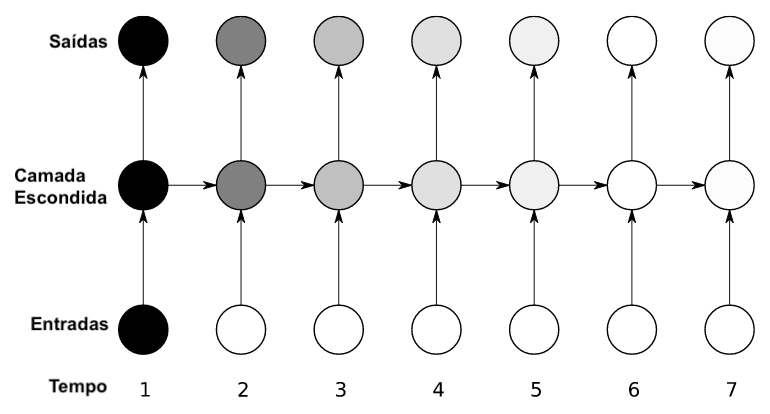
\includegraphics[scale=0.85]{resources/images/pln/rnn-vanishing-gradient.png}
        \smallcaption{Fonte: Autor \enquote{adaptado de} \citefloat{Graves2012Supervised}, p. 32.}
        \label{fig:rnn-vanishing-gradient}
\end{figure}

A arquitetura da \glsxtrfull{lstm} é composta por blocos de memória conectados recorrentemente, o que diminui o efeito de desvanecimento de gradiente. Cada bloco possui uma célula de memória e unidades multiplicativas, sendo elas: a entrada, a saída e o esquecimento. Essas células trabalham habilitando ou inibindo sinais provenientes de suas origens, podendo acessar informações através de um longo período de tempo. A Figura \ref{fig:rnn-lstm-memoria} apresenta um bloco de memória com uma única célula.
\begin{figure}[htbp]
    \centering
        \caption[Bloco de memória da \glsxtrfull{lstm} com uma célula.]{Bloco de memória da \glsxtrfull{lstm} com uma célula. As portas controlam a ativação das células através de multiplicação, sendo que as portas de entrada e saída multiplicam a entrada e saída da célula e a porta de esquecimento controla o estado anterior da própria célula. As portas são unidades somatórias não lineares, e a função $f$ é usualmente uma função sigmoide sendo o limite inferior 0 e o superior 1, representando os estados fechado e aberto, respectivamente. As funções de entrada e saída, $g$ e $h$, são normalmente tangentes hiperbólicas ou funções sigmoides, podendo a saída ser uma função identidade. As linhas tracejadas entre a célula e as portas são ponderadas, enquanto todas as outras conexões não são, ou seja, possuem peso igual a $1.0$.}
        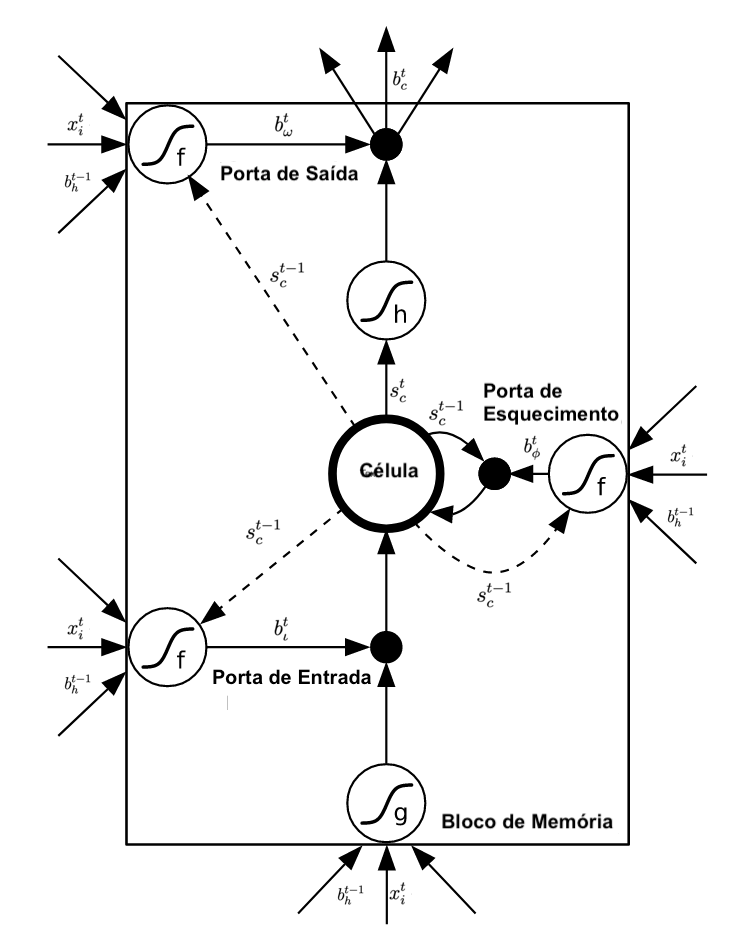
\includegraphics[scale=0.8]{resources/images/pln/rnn-lstm-memoria.png}
        \smallcaption{Fonte: Autor \enquote{adaptado de} \citefloat{Graves2012Supervised}, p. 33.}
        \label{fig:rnn-lstm-memoria}
\end{figure}

Uma sequência $x$ de comprimento $T$ pode ser recursivamente calculada durante a passagem direta aplicando as equações \ref{eq:lstm-input-gates}, \ref{eq:lstm-forget-gates}, \ref{eq:lstm-cells}, \ref{eq:lstm-output-gates} e \ref{eq:lstm-output}, na ordem que é apresentada, iniciando no instante $t =1$ até $T$ incrementalmente \cite{Graves2012Supervised}.

Foi considerado na Equação \ref{eq:lstm-input-gates} que $w_{ij}$ é o peso da conexão da unidade $i$ para $j$, a entrada da rede da unidade $j$ no instante $t$ é $a_j^t$ e $b_j^t$ a ativação da unidade $j$ no instante $t$. As portas de entrada, esquecimento e saída são referenciadas utilizando as subscrições $\iota$, $\phi$, $\omega$. A célula de memória é denotada por $c$ e suas influências sobre as portas são representadas por $w_{c\iota}$, $w_{c\phi}$ e $w_{c_\omega}$. O estado da célula $c$ no instante $t$ é definido por $s_c^t$, $f$ é a função de ativação das portas e $g$ e $h$ a função de ativação da entrada e saída, respectivamente. $I$ é o número de entradas, $H$ o número de células na camada escondida e $C$ é o número de células. Apenas as saídas das célula $b_c^t$ são conectadas a outros blocos e os índices $h$ fazem referência às saídas de outra célula da camada escondida.

Portas de Entrada:
\begin{equation}
\begin{split}
    \label{eq:lstm-input-gates}
    & a_\iota^t = \sum_{i=1}^{I} w_{i\iota} x_i^t
                  + \sum_{h=1}^{H} w_{h\iota} b_h^{t-1}
                  + \sum_{c=1}^{C} w_{c\iota} s_c^{t-1} \\
    & b_\iota^t = f(a_\iota^t)
\end{split}
\end{equation}

Portas de Esquecimento:
\begin{equation}
\begin{split}
    \label{eq:lstm-forget-gates}
    & a_\phi^t = \sum_{i=1}^{I} w_{i\phi} x_i^t
                 + \sum_{h=1}^{H} w_{h\phi} b_h^{t-1}
                 + \sum_{c=1}^{C} w_{c\phi} s_c^{t-1} \\
    & b_\phi^t = f(a_\phi^t)
\end{split}
\end{equation}

Células:
\begin{equation}
\begin{split}
    \label{eq:lstm-cells}
    & a_c^t = \sum_{i=1}^{I} w_{ic} x_i^t
              + \sum_{h=1}^{H} w_{hc} b_h^{t-1} \\
    & s_c^t = b_\phi^t s_c^{t-1} + b_\iota^t g(a_c^t)
\end{split}
\end{equation}

Portas de Saída:
\begin{equation}
\begin{split}
    \label{eq:lstm-output-gates}
    & a_\omega^t = \sum_{i=1}^{I} w_{i\omega} x_i^t
                   + \sum_{h=1}^{H} w_{h\omega} b_h^{t-1}
                   + \sum_{c=1}^{C} w_{c\omega} s_c^{t-1} \\
    & b_\omega^t = f(a_\omega^t)
\end{split}
\end{equation}

Saídas da Célula:
\begin{equation}
\begin{split}
    \label{eq:lstm-output}
    & b_c^t = b_\omega^t h(s_c^t)
\end{split}
\end{equation}

\subsubsection{\glsentrylong{bi-lstm}}
\label{sec:bilstm}

Para aplicações em que toda a sentença está disponível antes da produção do resultado, a utilização do contexto passado (à esquerda da posição atual) quanto do contexto futuro (à direita da posição atual) podem apresentar um desempenho superior se comparada a utilizado apenas o contexto passado. Por exemplo, considere as frases (1) \enquote{Ele disse: Oliveira e Pereira são senhores alegres} e (2) \enquote{Ele disse: Oliveira e Pereira são árvores não originárias do Brasil}. Considere também que cada palavra, delimitada por espaços ou pontuações, são \textit{tokens} que variam de $1$ a $N$. As posições $t_4$ e $t_6$ possuem as mesmas palavras em ambas as sentenças, mas no caso (1) se referem a nomes ou sobrenomes de pessoas, enquanto que no caso (2) se referem a tipos de árvores. Para saber se essas posições são relacionadas a nomes ou tipos de árvores é necessário verificar as posições $t_7$ e $t_8$ que, em ambos os casos, estão à direita das palavras alvo.

O acesso futuro poderia ser realizado através de um janelamento, semelhante ao apresentado no modelo de vetorização de palavras \textit{Skip-Gram} (Seção \ref{sec:word-embedding-sg}), porém sofreria da limitação de alcance fixo do contexto, podendo não capturar os detalhes necessários dependendo da largura pré-definida da janela.

As \glsxtrfullpl{bi-lstm} apresentam uma forma de preservar tanto o contexto futuro quanto o passado, através do treinamento de forma direta e reversa, utilizando duas camadas recorrentes separadamente, conectando-as a uma mesma unidade de saída, conforme a Figura \ref{fig:rnn-bidirecionalidade}. Tal bidirecionalidade não é exclusiva da \gls{lstm}, mas pode ser ampliada para as redes \gls{rnn} de forma generalizada. \cite{Graves2012Supervised}

\begin{figure}[htbp]
    \centering
        \caption[Rede \glsxtrfull{rnn} bidirecional desenrolada.]{Rede \glsxtrfull{rnn} bidirecional desenrolada. Os mesmos conjuntos de pesos são reutilizados a cada passo de tempo e a entrada da camada de saída são os estados escondidos da camada direta e da reversa, não havendo interlocução entre as camadas intermediárias.}
        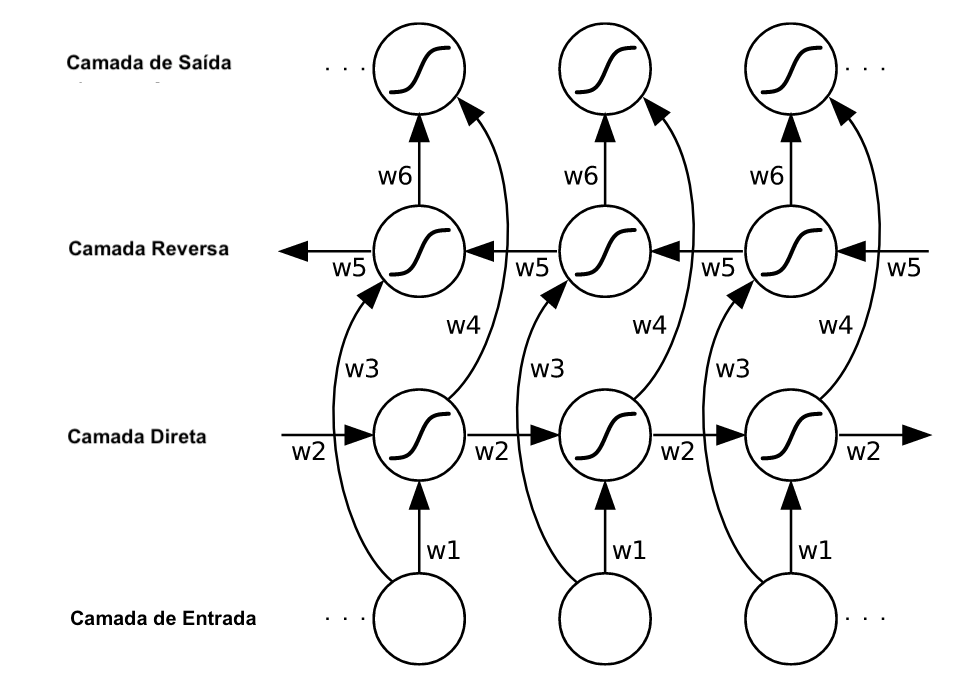
\includegraphics[scale=0.8]{resources/images/pln/rnn-bidirecionalidade.png}
        \smallcaption{Fonte: Autor \enquote{adaptado de} \citefloat{Graves2012Supervised}, p. 22.}
        \label{fig:rnn-bidirecionalidade}
\end{figure}

\subsection{\glsentrylong{gru}}
\label{sec:gru}

As \glsxtrfullpl{gru} são mais simples do que as \glspl{lstm} em termos de facilidade de implementação e uso de recursos computacionais. Elas foram introduzidas por \textcite{Cho2014Learning} e possuem duas portas, a de atualização e a de reinicialização, sendo a primeira descrita pela Equação \ref{eq:gru-update} e a outra pela \ref{eq:gru-reset}. As equações representam a $j$-ésima unidade escondida, sendo $\sigma$ a função logística sigmoide, $[\vec v]_j$ o $j$-ésimo elemento do vetor $\vec v$, $x$ e $h_{(t-1)}$ a entrada e o estado escondido anterior e $W$ e $U$ as matrizes de pesos que são aprendidas. A ativação atual da unidade $h_j$ é descrita pela Equação \ref{eq:gru-activation}.
\begin{equation}
    \label{eq:gru-update}
    r_j = \sigma([W_r x]_j + [U_r h^{(t-1)}]_j)
\end{equation}
\begin{equation}
    \label{eq:gru-reset}
    z_j = \sigma([W_z x]_j + [U_z h^{(t-1)}]_j)
\end{equation}
\begin{equation}
    \label{eq:gru-activation}
    h_j^t = z_j h_j^{(t-1)} + (1 - z_j) \tilde{h}_j^t
\end{equation}
\begin{equation}
    \label{eq:gru-activation-tild}
    \tilde{h}_j^t = \phi([Wx]_j + [U(r \odot h^{(t-1)})]_j)
\end{equation}

Podemos entender, portanto, que a porta de reinicialização controla a quantidade de informações do estado escondido anterior em relação a entrada que flui para o estado escondido atual. Quando seu valor é próximo a 0, o estado escondido tende a absorver mais informações da entrada do que do estado anterior; quando seu valor é próximo a 1, o estado atual será composto, em sua maioria, por informações do estado atual. A porta de atualização controla a quantidade de informação que será carregada do estado escondido anterior para o atual, ajudando a preservar dados de longo alcance.

Cada unidade escondida contém suas próprias portas, o que permite que capturem dependência temporais diferentes. Quando a dependência temporal é de curto alcance, a porta de reinicialização fica ativa por um período de tempo maior, por outro lado, quando há uma dependência de longo alcance, a porta de atualização é ativada com maior frequência.

A Figura \ref{fig:lstm-vs-gru} apresenta uma versão simplificada da \gls{lstm} e da \gls{gru}. Diferente das \glspl{rnn} tradicionais, em que o sinal de ativação é substituído com o resultado do cálculo que utiliza a entrada e o estado escondido anterior, nesses dois modelos há um componente aditivo de sua atualização de $t$ para $t + 1$, podendo criar um caminho temporal mais curto diminuindo o desvanecimento de gradiente durante a propagação reversa do erro \cite{Chung2014Empirical}.

\begin{figure}[htbp]
    \centering
        \caption[Comparativo entre a \glsxtrfull{lstm} e a \glsxtrfull{gru}.]{(a) \glsxtrfull{lstm} e (b) \glsxtrfull{gru}. Em que $i$, $f$, $o$ da figura (a) representam as portas de entrada, esquecimento e saída; $c$ é o estado atual da célula e $\tilde{c}$ o estado futuro. As variáveis $r$ e $z$, da figura (b), são as portas de reinicialização e atualização; $h$ e $\tilde{h}$ são a ativação e a ativação candidata futura.}
        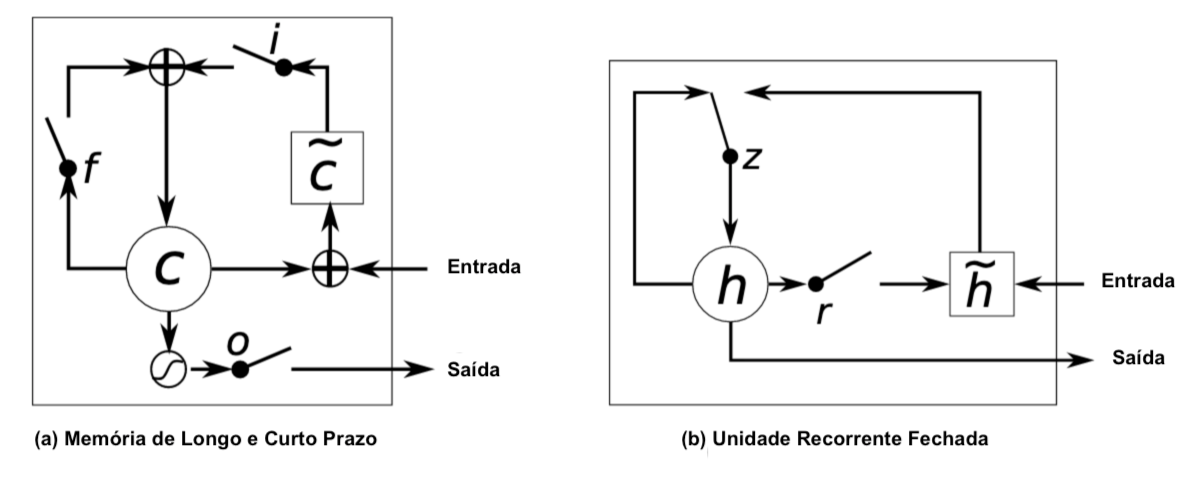
\includegraphics[width=\textwidth]{resources/images/pln/lstm-vs-gru.png}
        \smallcaption{Fonte: Autor \enquote{adaptado de} \citefloat{Chung2014Empirical}, p. 3.}
        \label{fig:lstm-vs-gru}
\end{figure}

\subsection{Codificador-Decodificador}
\label{sec:encoder-decoder}

Codificadores-decodificadores são uma família de modelos que aprendem a mapear dados em um domínio de entrada para um domínio de saída através de uma rede com dois estágios \cite{Minaee2020Image}.

\textcite{Bahdanau2016Neural} apresentaram uma abordagem comum de codificadores-decodificadores com \gls{rnn} como uma sequência de vetores $X = (x_1, \dots, x_{T_x})$, lidos pelo codificador em um vetor $c$, conforme equações \ref{eq:enc-dec-hidden} e \ref{eq:enc-dec-latent-state}, em que $h_t \in \mathbb{R}^n$ é o estado escondido no tempo $t$ e $f$ e $q$ são funções não lineares.
\begin{equation}
    \label{eq:enc-dec-hidden}
    h_t = f(x_t, h_{t-1})
\end{equation}
\begin{equation}
    \label{eq:enc-dec-latent-state}
    c = q(\{ h_1, \dots, h_{T_x} \})
\end{equation}

O decodificador, normalmente treinado para predizer a próxima palavra $y_{t^\prime}$ dado um vetor de contexto $c$ e todas as predições anteriores $Y = \{y_1, \dots, y_{t^\prime - 1}\}$, é descrito pela Equação \ref{eq:enc-dec-prob-output} e, para o caso da \gls{rnn}, cada probabilidade condicional é modelada conforme Equação \ref{eq:enc-dec-rnn-prob-output}, em que $g$ é uma função não linear que fornece uma probabilidade de saída $y_t$, $s_t$ é o estado escondido da \gls{rnn}.
\begin{equation}
    \label{eq:enc-dec-prob-output}
    p(Y) = \prod_{t=1}^{T} p(y_t | \{ y_1, \dots, y_{t-1} \}, c)
\end{equation}
\begin{equation}
    \label{eq:enc-dec-rnn-prob-output}
    p(y_t | {y_1, \dots, y_{t-1}}, c) = g(y_{t-1}, s_t, c)
\end{equation}

De forma mais simples, o codificador comprime uma entrada $x$, através de uma função de codificação $f$, em uma representação do espaço latente $c$, sendo $c = f(x)$. O decodificador busca maximizar a probabilidade da saída $y$, utilizando o espaço latente e uma função de decodificação $g$, sendo $y = g(c)$.

A representação do espaço latente é capaz de capturar informações semânticas da entrada úteis para predizer a saída e pode ser entendida como a representação de vetores de atributos. Tais sistemas são usualmente treinados minimizando a perda na reconstrução $L(y, \hat{h})$ entre a saída esperada e a estimada. A Figura \ref{fig:encoder-decode-rnn} ilustra um bloco de codificação-decodificação que utiliza \gls{rnn}. Codificadores próprios (\textit{autoencoder}) são um tipo especial em que a saída é a mesma que a entrada.
\begin{figure}[htbp]
    \centering
        \caption[Codificador-Decodificador utilizando \glsxtrfull{rnn}.]{Codificador-Decodificador utilizando \glsxtrfull{rnn}. As entradas $(x_1, x_2, \dots, x_T)$ são recorrentemente lidas produzindo o estado latente $c$, que é então utilizado pelo decodificador para produzir a sequência de saída $(y_1, y_2, \dots, y_{T^\prime})$}
        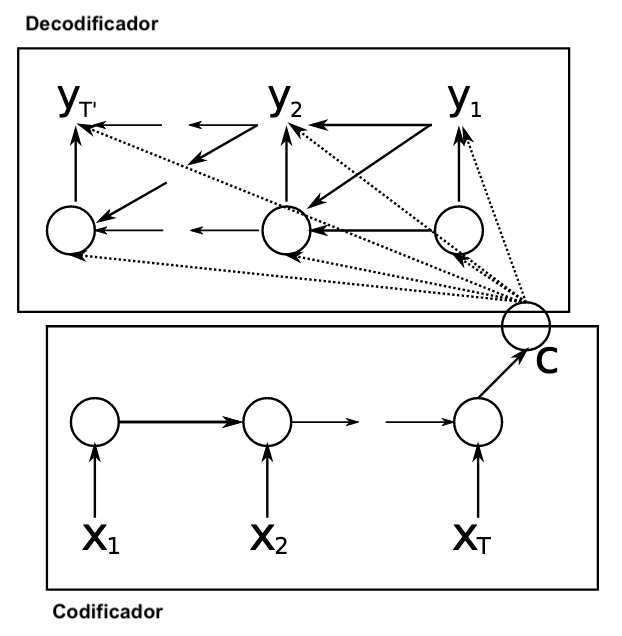
\includegraphics[scale=0.85]{resources/images/pln/encoder-decoder-rnn.png}
        \smallcaption{Fonte: Autor \enquote{adaptado de} \citefloat{Cho2014Learning}, p. 2.}
        \label{fig:encoder-decode-rnn}
\end{figure}

\subsubsection{Modelo de Atenção}
\label{sec:encoder-decoder-attention}

As \glsxtrfullpl{nmt} buscam construir uma única rede neural em que seu treinamento é realizado em conjunto, maximizando seu desempenho. Pertencentes a família de codificadores-decodificares, elas transformam uma sentença de entrada em um vetor de tamanho fixo que é então utilizado para produzir a tradução.

A utilização de um vetor de tamanho fixo impõe uma limitação à capacidade de produção de saídas, já que a representação latente deve possuir informação suficiente pra a inferência de sentenças. Buscando otimizar esse problema, \textcite{Bahdanau2016Neural} propuseram uma extensão ao modelo, tornando-o capaz de buscar por partes da sentença de entrada relevantes para a predição de uma palavra de saída.

A busca por partes da sentença de entrada foi chamada, intuitivamente, de atenção. Desse modo, o decodificador decide quais partes da sentença de entrada ele deve prestar atenção, diminuindo a necessidade de o codificador produzir um único espaço latente contendo todas as informações. Essa abordagem faz com que a informação possa ser espalhada, através de anotações, por toda a sequência de entrada, deixando a cargo do decodificador a seleção de quais anotações são importantes para um determinado momento \cite{Bahdanau2016Neural}. A Figura \ref{fig:rnn-attention} exemplifica um codificador-decodificador com \gls{rnn} bidirecional com atenção. A bidirecionalidade foi apresentada na Seção \ref{sec:bilstm}. 
\begin{figure}[htbp]
    \centering
        \caption[Codificador-Decodificador utilizando \glsxtrfull{rnn} bidirecional com mecanismos de atenção.]{Codificador-Decodificador com \glsxtrfull{rnn} bidirecional com atenção, produzindo a t-ésima palavra alvo $y_t$ dado uma sentença de entrada $x_1, x_2, \dots x_T$. Os espaços escondidos $a_{t,1}, a_{t,2}, \dots, a_{t,T}$ produzidos pelo codificador, são utilizados como anotações para o mecanismo de atenção e, juntamente com a palavra alvo anterior $y_{t-1}$, a predição é realizada pelo decodificador.}
        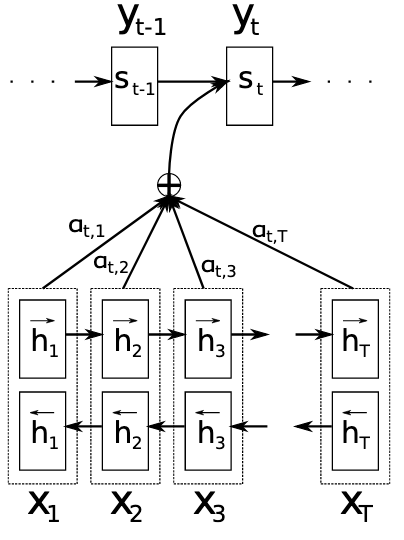
\includegraphics[scale=0.85]{resources/images/pln/rnn-attention.png}
        \smallcaption{Fonte: \citefloat{Bahdanau2016Neural}, p. 3.}
        \label{fig:rnn-attention}
\end{figure}

Utilizando as mesmas equações da Seção \ref{sec:encoder-decoder} como base para a extensão, a probabilidade condicional definida na Equação \ref{eq:enc-dec-prob-output} foi reescrita conforme \ref{eq:enc-dec-attention}:
\begin{equation}
    \label{eq:enc-dec-attention}
    p(i_t | \{ i_1, \dots, y_{i-1} \}, X) = g(y_{i-1}, s_i, c_i)
\end{equation}
em que $s_i$ é o estado escondida da \gls{rnn} no instante $i$, caracterizado pela Equação \ref{eq:enc-dec-attention-hidden-state}.
\begin{equation}
    \label{eq:enc-dec-attention-hidden-state}
    s_i = f(s_{i-1}, y_{i-1}, c_i)
\end{equation}

Diferentemente dos codificadores-decodificados comuns, cada probabilidade condicional possui um contexto $c_i$ distinto para cara palavra alvo $y_i$, sendo que o contexto depende de uma sequência de anotações $h_1, \dots, h_{T_x}$ produzidas pelo codificador para cada entrada $x_i$. O contexto $c_i$ é computado como uma soma ponderada das anotações conforme Equação \ref{eq:enc-dec-attention-context}. E o peso $\alpha_{i,j}$ para cada anotação $h_j$ é descrito pelas equações \ref{eq:enc-dec-attention-context-weigth} e \ref{eq:enc-dec-attention-context-weigth-energy}.
\begin{equation}
    \label{eq:enc-dec-attention-context}
    c_i = \sum_{j = 1}^{T_x} \alpha_{i,j} h_j
\end{equation}
\begin{equation}
    \label{eq:enc-dec-attention-context-weigth}
    \alpha_{i,j} = \frac{exp(e_{i,j})}{\sum_{k=1}^{T_x}exp(e_{i,j})}
\end{equation}
\begin{equation}
    \label{eq:enc-dec-attention-context-weigth-energy}
    e_{i,j} = a(s_{i-1}, h_j)
\end{equation}

A Equação \ref{eq:enc-dec-attention-context-weigth-energy} descreve o quão bem as entradas ao redor da j-ésima posição de entrada e a i-ésima saída se relacionam. A função $a$ pode ser parametrizada através de uma \gls{ffn} que é treinada em conjunto com outros componentes do sistema.

\subsection{\textit{Transformer}}
\label{sec:transformer}

O \textit{Transformer}, apresentado por \textcite{Vaswani2017Attention}, é um modelo de transdução sequencial composto por um codificador e decodificador baseados inteiramente em modelos de atenção, substituindo camadas de recorrência por atenção própria multifacetada. Os codificadores-decodificadores foram apresentados na Seção \ref{sec:encoder-decoder}, o modelo de atenção na Seção \ref{sec:encoder-decoder-attention}, e a redes recorrentes nas seções \ref{sec:rnn}, \ref{sec:lstm} e \ref{sec:gru}.

Essa arquitetura segue a abordagem do codificar-decodificador, em que uma sequência de entrada $(x_1, \dots, x_n)$ é mapeada para uma sequência contínua de representações $z = (z_1, \dots, z_n)$ e então, o decodificador, utilizando $z$, produz uma sequência de símbolos $(y_1, \dots, y_m)$, um por vez, utilizando o símbolo gerado anteriormente como entrada adicional.

O \textit{Transformer} utiliza um empilhamento de atenção próprio e camadas completamente conectadas tanto para o codificador quanto para o decodificador. O modelo de arquitetura do codificador e decodificador é apresentado na Figura \ref{fig:transformer-arquitetura}.
\begin{figure}[htbp]
    \centering
        \caption[Modelo de arquitetura do \textit{Transformer}.]{Modelo de arquitetura do \textit{Transformer}. Do lado esquerdo o codificador, em que a entrada são \textit{embeddings}, seguidos por um codificador posicional, e $Nx$ camadas, cada qual composta por atenção multifacetada seguida por uma rede \gls{ffn}. Do lado direito o decodificador, com os \textit{embeddings} de saída, o codificador posicional, seguido por $Nx$ camadas, compostas por atenção mascaradas multifacetada, um mecanismo de atenção entre o decodificador e codificador e uma rede \gls{ffn}. As probabilidades de saídas são calculadas através da linearização e \textit{softmax}.}
        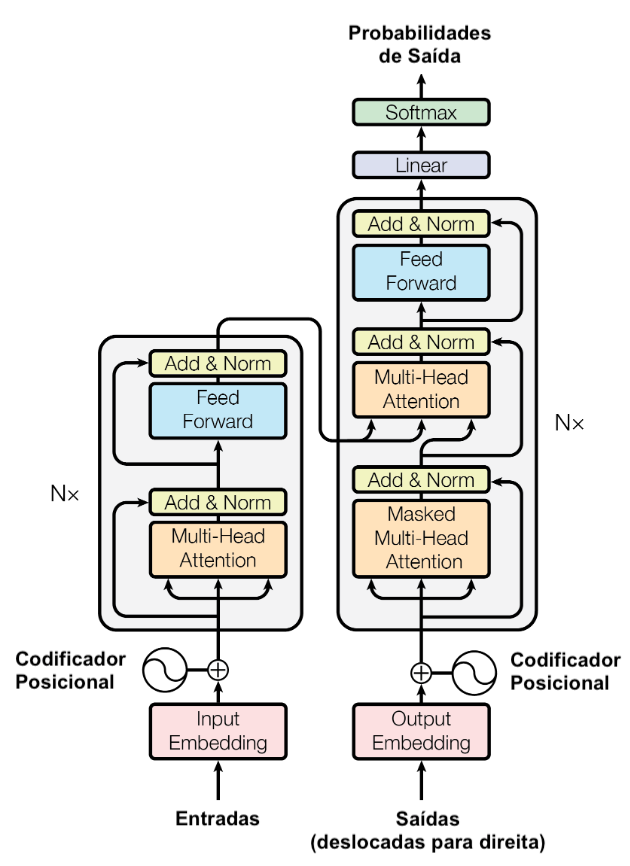
\includegraphics[scale=0.85]{resources/images/pln/transformer.png}
        \smallcaption{Fonte: Autor \enquote{adaptado de} \citefloat{Vaswani2017Attention}, p. 3.}
        \label{fig:transformer-arquitetura}
\end{figure}

O codificador é composto por $N = 6$ camadas idênticas empilhadas paralelamente, cada qual contendo duas subcamadas. A primeira contém um mecanismo de atenção própria multifacetada e a segunda uma rede \gls{ffn} totalmente conectada. Cada subcamada possui mecanismos de conexão residual e normalização, fazendo com que sua saída seja $\textit{normalização}(x + \textit{subcamada}(x))$, em que $\textit{subcamada}(x)$ é a função da subcamada. Para simplificar a conexão residual, todas as subcamadas e as camadas de \textit{embedding} produzem dimensões de saída $d_{model} = 512$.

O decodificador também é composto pelo mesmo número de camadas que o codificador. Além das duas subcamadas do codificador, o decodificador adiciona uma terceira que realiza a atenção multifacetada na saída do empilhamento do codificador. Para cada subcamada, o decodificador também realiza a normalização e conexão residual. A subcamada de atenção própria é ligeiramente diferente da subcamada do codificador devido a necessidade de prevenir o decodificador de se atentar a posições subsequentes. Essa diferença é realizada através do mascaramento dos elementos posteriores, o que, juntamente com o deslocamento de uma posição, garante que uma predição para a posição $i$ dependa somente das posições conhecidas até o momento anterior a $i$.

Mapear uma pergunta $Q$, a um conjunto de pares de chaves-valores $(K, V)$ e a uma saída, é a base do mecanismo de atenção do \textit{Transformer}. Os elementos desse mapeamento são todos vetores, e a saída é uma soma ponderada de todos os valores, a ponderação é uma função de compatibilidade entre $Q$ e $K$.

A Figura \ref{fig:transformer-atencao-produto-escalar-ajustado} apresenta o processo de cálculo de atenção com produto escalar ajustado. Sua entrada são $Q$ e $K$ de dimensão $d_k$, e $V$ com dimensão $d_v$. O produto escalar da pergunta com todas as chaves são computados e divididos por $\sqrt{d_k}$, a distribuição de probabilidade é então calculada através do \textit{softmax} para então gerar o peso de cada valor. Sua forma matricial, utilizada principalmente para múltiplas perguntas $Q$, é exibida na Equação \ref{eq:transformer-attention}. O ajuste do produto escalar por $\frac{1}{\sqrt{d_k}}$ é devido ao seu resultado ficar muito elevado quando $d_k$ é grande, fazendo o \textit{softmax} atingir regiões onde seu gradiente é muito pequeno.
\begin{equation}
    \label{eq:transformer-attention}
    \text{Atenção}(Q, K, V) = softmax \left( \frac{QK^T}{\sqrt{d_k}} \right) V
\end{equation}

\begin{figure}[htbp]
    \centering
        \caption{Atenção com produto escalar ajustado.}
        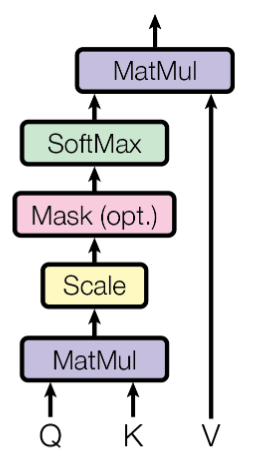
\includegraphics[scale=0.85]{resources/images/pln/transformer-scaled-dot-product-attention.png}
        \smallcaption{Fonte: \citefloat{Vaswani2017Attention}, p. 4.}
        \label{fig:transformer-atencao-produto-escalar-ajustado}
\end{figure}

A atenção multifacetada ocorre pela projeção linear das perguntas, chaves e valores $h$ vezes, ao invés de computar a atenção em uma única função com dimensão $d_{\text{model}}$. O processamento após a projeção ocorre paralelamente, resultando em valores de saída com dimensão $d_v$, que são concatenados e projetados novamente resultando nos valores finais conforme Figura \ref{fig:transformer-atencao-multifacetada}.

\begin{figure}[htbp]
    \centering
        \caption{Atenção multifacetada.}
        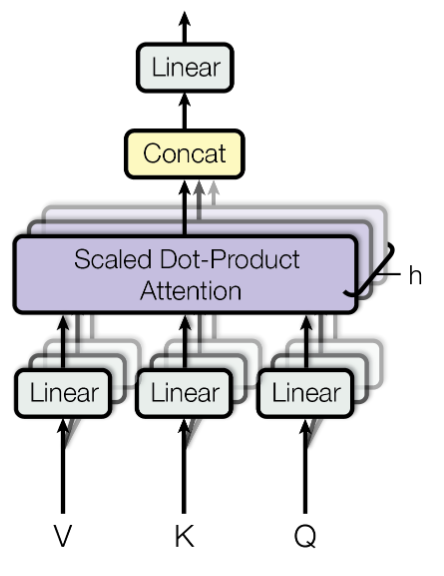
\includegraphics[scale=0.85]{resources/images/pln/transformer-atencao-multifacetada.png}
        \smallcaption{Fonte: \citefloat{Vaswani2017Attention}, p. 4.}
        \label{fig:transformer-atencao-multifacetada}
\end{figure}

As equações \ref{eq:transformer-multi-head} e \ref{eq:transformer-multi-head-attention-i} apresentam o multifacetamento. As projeções lineares são matrizes $W_i^Q \in \mathbb{R}^{d_{model} \times d_k}$, $W_i^K \in \mathbb{R}^{d_{model} \times d_k}$, $W_i^V \in \mathbb{R}^{d_{model} \times d_v}$ e $W^O \in \mathbb{R}^{hd_v \times d_{model}}$.
\begin{equation}
    \label{eq:transformer-multi-head}
    \textit{Multifacetamento}(Q, K, V) = concat(\textit{faceta}_1, \dots, \textit{faceta}_h)W^O
\end{equation}
\begin{equation}
    \label{eq:transformer-multi-head-attention-i}
    \textit{faceta}_i = \textit{Atenção}(QW_i^Q, KW_i^K, VW_i^V)
\end{equation}

A segunda subcamada do codificador, ou a terceira do decodificador, contém uma rede \gls{ffn} totalmente conectada. Ela é aplicada a cada posição de entrada separadamente, porém de forma idêntica, isto é, a transformação linear é a mesma entre as diferentes posições de uma mesma camada, porém diferentes parâmetros são usados em diferentes camadas. A rede consiste em duas transformações lineares com uma ativação \textit{ReLu} entre elas, conforme Equação \ref{eq:transformer-ffn}. Tanto a entrada quanto a saída possuem dimensão $d_{model} = 512$.
\begin{equation}
    \label{eq:transformer-ffn}
    FFN(x) = max(0, xW_1 + b1)W_2 + b_2
\end{equation}

O codificador posicional é utilizado para prover informações sobre a ordem da sequência, já que o modelo não possui recorrência ou convolução. O posicionamento é realizado adicionando informações nos \textit{embeddings} de entrada e saída. O codificador posicional pode ser aprendido ou ser fixo, sendo que o modelo apresentado por \textcite{Vaswani2017Attention} possui codificado fixo.

\textcite{Vaswani2017Attention} comparou a atenção próprio com a recorrência e convolução em três aspectos: complexidade computacional total por camada, possibilidade de paralelização da computação através de do número mínimo de operações sequenciais e comprimento do caminho em dependências de longo alcance.

A Tabela \ref{table:transformer-comparison} apresenta o resultado dessa comparação. A atenção própria conecta todas as posições com um número constante de operações, enquanto a recorrente necessita de $O(n)$ operações. A atenção própria também é mais eficiente em termos de complexidade computacional, do que a recorrente quando o comprimento da sequência $n$ é menor do que a dimensão da representação $d$, o que é usual nos modelos de \gls{nmt}. Caso seja necessário melhorar o desempenho para sequências longas, a atenção própria pode ser restringida em um contexto de tamanho $r$, o que aumentaria o comprimento do caminho máximo para $O(n/r)$.

\begin{table}[ht!]
    \caption[Desempenho de diferentes modelos de aprendizado.]{Máximo comprimento do caminho, complexidade por camada e número mínimo de operações sequencias para diferentes tipos de camadas. A variável $n$ é o comprimento da sentença, $d$ é a dimensão da representação, $k$ é o tamanho do \textit{kernel} e $r$ o tamanho do contexto da atenção própria restrita.}
    \label{table:transformer-comparison}
    \centering
    \begin{tabular}{p{4.2cm}|p{3cm}|p{2.5cm}|p{4cm}}
        \hline
        Tipo de Camada              & Complexidade por Camada   & Operações Sequências  & Comprimento Máximo do Caminho \\
        \hline
        Atenção Própria             & $O(n^2.d)$                & $O(1)$                & $O(1)$ \\
        \hline
        Recorrente                  & $O(n.d^2)$                & $O(n)$                & $O(n)$ \\
        \hline
        Convolucional               & $O(k,b,d^2)$              & $O(1)$                & $O(\log_k(n))$ \\
        \hline
        Atenção Própria Restrita    & $O(r.n.d)$                & $O(1)$                & $O(\frac{n}{r})$ \\
        \hline
    \end{tabular}
    \smallcaption{Fonte: \citefloat{Vaswani2017Attention}}
\end{table}

\section{DISCUSSÃO}
\label{sec:pln-discussion}

Um dos grandes desafios do \glsxtrfull{pln} é a representação das palavras. Áreas como linguística e psicologia ajudam a entender o relacionamento entre elas. Esse relacionamento possui diversas dimensões e dependem de particularidades de cada idioma. Porém, a dimensionalidade de suas representações pode tornar o processamento computacionalmente inviável. Para isso, faz-se necessária a representação de palavras em um conjunto reduzido de dimensões.

Tal conjunto reduzido de dimensões é conhecido como \textit{word embedding}. Essa redução dimensional busca capturar similaridades semânticas e sintáticas entre palavras ou até mesmo frases. As similaridades então ajudam a encontrar formas linguísticas dado um domínio de palavras.

O \textit{word embedding} são normalmente representações vetoriais de palavras. Tais representações vetoriais são utilizadas na camada de entrada de diversas tarefas de \gls{pln}. Normalmente, tais tarefas são treinadas de forma supervisionadas, ao contrário do \textit{word embedding}, que é treinado de forma não supervisionado, utilizando grandes \textit{corpora} de dados.

Uma das importâncias do \textit{word embeddings} é relacionada à hipótese distribucional, que afirma que palavras de alta relação aparecem em contextos linguísticos semelhantes. Desse modo, a representação vetorial fornece meios de encontrar relacionamento entre palavras considerando um número limitado de dimensões.

A capacidade da representação vetorial pode ser avaliada em dois aspectos diferentes. O primeiro é a aplicação direta do \textit{word embedding} em tarefas de \gls{pln}, e assim comparar os diferentes resultados das diferentes representações vetoriais. Um desafio a essa abordagem é a dificuldade de generalização, ou seja, é difícil determinar se uma representação vetorial desempenha melhor do que outra sem avaliar sua aplicação em uma coleção de tarefas específicas. Os métodos intrínsecos, por outro lado, possuem uma generalização mais abrangente, pois os avaliadores não dependem de tarefas específicas. Porém, não há garantias que uma tarefa específica terá um desempenho melhor quando utilizada representações vetoriais com um relacionamento semântico e sintático superior.

Diversos métodos de treinamento de representações vetoriais foram propostos. Destacam-se o Word2Vec, GloVe e FastText. O Word2Vec é um método que utiliza um contexto limitado para treinar representações de palavras. Tal contexto corresponde a palavras imediatamente anteriores e imediatamente posteriores. Esse contexto representa uma abordagem estatística não ótima.

O modelo GloVe foi concebido buscando adicionar relações semânticas e sintáticas a uma abordagem que utiliza uma base estatística sólida. Para isso, foi utilizada a razão entre a probabilidade de pares de palavras coocorrerem no corpus.

O modelo FastText, podendo ser considerado uma extensão do Word2Vec, possui a capacidade de representar palavras raras. Para isso, cada palavra é dividida em partes, a composição vetorial de todas as partes que compõem uma dada palavra resulta no vetor da palavra alvo. Assim, diferenças morfossintáticas entre as palavras podem ser representadas.

Esses modelos de representação vetoriais são considerados estáticos, ou seja, apresentam um mesmo vetor para uma dada palavra, independentemente do contexto. Também existem os métodos de vetorização de palavras contextualizados, que podem possuir mais do que uma única representação vetorial para uma mesma palavra dependendo do contexto que ela está inserida. Técnicas conhecidas como aprendizado em conjunto utilizam junções de \textit{embeddings} estáticos e contextualizados a fim de melhorarem seu desempenho.

Independente da vetorização de palavras, existe uma etapa de pré-processamento conhecida como \textit{tokenização}. Ela é responsável por transformar um texto em termos. Os termos podem ser palavras, o que leva a uma situação onde palavras raras podem não aparecer no conjunto de treinamento e, consequentemente, não ser reconhecida nos processos subsequentes de \gls{pln}. Alguns métodos de vetorização, como o FastText, lidam com essa característica, porém, \textit{tokenizadores} subpalavras podem ser utilizados para minimizar tal condição.

Os \textit{tokenizadores} subpalavras possuem a necessidade de escolha dos melhores \textit{tokens} para compor uma palavra. Tal escolha pode aumentar a probabilidade máxima do \gls{ml}, como o WordPiece, ou ser completamente determinístico, como o \gls{ml} uni-grama.

Qualquer que seja o caso, presunções podem afetar a aplicabilidade do modelo em diferentes idiomas. Por exemplo, alguns idiomas asiáticos podem não utilizar o espaço, em certas situações, como separador de palavras; idiomas europeus utilizam uma junção de espaço ou caracteres de pontuação como divisores de palavras.

O SentencePiece, um \textit{tokenizador} subpalavra sem perdas e autocontido, não assume que palavras são separadas por espaços, e treinam seu \gls{ml} a partir dos dados com o mínimo de pré-processamento. Qualquer que seja o processamento, seu modelo é combinado juntamente com o vocabulário, de tal forma que ele possa ser utilizado sem ambiguidade por outras aplicações. Tais características torna-o robusto para lidar com palavras raras.

Usualmente, o corpus utilizado em tarefas de \gls{pln} é pré-processado, \textit{tokenizado}, e suas representações vetoriais geradas antes deles serem utilizados como entrada de redes neurais artificias, podendo influenciar o desempenho final de aplicações específicas.

Algumas aplicações de \gls{pln}, como a \gls{nmt}, utilizam de codificadores-decodificadores para produzirem uma ou mais saídas dada uma sequência de entrada através de uma arquitetura de dois estágios. Modelos de aprendizado profundo podem ser utilizados de forma independente entre os estágios de codificação e decodificação.

Uma notória família de modelos de aprendizado profundo é a \gls{rnn}, que utiliza da recursão para comprimir a entrada em espaços semânticos latentes, um passo por \textit{token}. Essas codificações são então apresentadas ao decodificador que, sequencialmente, produzem o resultado que maximiza a probabilidade de um conjunto de \textit{tokens} de saída.

A \gls{rnn} sofre do problema de desvanecimento de gradiente, em que relacionamentos de longo alcance não são ajustados corretamente devido ao ganho, durante o treinamento, ser muito pequeno ao atravessar, recorrentemente, várias camadas. Visando minimizar esse problema, redes como a \gls{lstm} e a \gls{gru} podem ser utilizadas. Essas redes empregam a mesma ideia de recorrência, porém, adicionam portas de controle, permitindo ou bloqueando diferentes fluxos, aumentando consideravelmente a possibilidade de relacionamento de longo alcance.

As redes neurais da família da \gls{rnn} processam os textos, ou \textit{tokens}, na ordem de leitura usual, ou seja, da esquerda para a direita. Desse modo, apenas relacionamento entre \textit{tokens} presentes e passados são modelados. Para adicionar um possível relacionamento futuro, é necessário adicionar a bidirecionalidade, como a \gls{bi-lstm} ou a \gls{bi-gru}.

A bidirecionalidade é atingida através do uso de duas redes semelhantes durante a etapa da codificação, uma no sentido direto, da esquerda para a direita, e outra no sentido reverso, da direita para a esquerda. Os espaços semânticos latentes são então combinados, semelhante ao processo utilizado pelo aprendizado em conjunto. Esse espaço de estados é então utilizado pela etapa de decodificação.

A utilização de um único espaço de estados, entre o codificador e o decodificador, exige que as informações sejam embutidas em um vetor de dimensionalidade reduzida, limitando a representação textual disponível para o decodificador. Os modelos de atenção podem então serem utilizados de tal forma que, espaços latentes intermediários sejam empregados dependendo do estágio da decodificação. Desse modo, o decodificador pode aumentar ou diminuir a \enquote{atenção} dada a certas etapas da codificação.

Os modelos de atenção ganharam grande interesse recentemente, e uma arquitetura de rede neural baseada, em sua grande maioria, em atenção foi criada, o \textit{Transformer}. Essa arquitetura não utiliza nenhum tipo de recorrência, e grande parte de seu treinamento pode ser feito de forma paralela. Ao invés dos \textit{tokens} serem apresentados um a um, sequencialmente, todos os \textit{tokens} são apresentados de uma só vez, fazendo assim o comprimento máximo entre caminhos de palavras ser $O(1)$, diferentemente do \gls{rnn}, que é $O(n)$.

O \textit{Transformer} utiliza subcamadas de atenção multifacetada, onde perguntas são comparadas com chaves, e os valores dessas chaves, que mais se assemelham a essas perguntas, são utilizados como saída dessa subcamada. As saídas são então processadas por uma rede neural totalmente conectada (\gls{ffn}).

Ambos, codificador e decodificador, utilizam atenção própria, em que a entrada para a pergunta, chave e valor são as mesmas. Adicionalmente, o decodificador, em uma subcamada adicional, utiliza um mecanismo de atenção aplicando a saída do codificador como entrada para a chave e o valor, e a saída de sua subcamada de atenção própria como pergunta.

O codificador e decodificador podem ser aninhados, ou seja, podem existir $N$ camadas de cada um deles. Porém, a quantidade de parâmetros para treinamento pode se tornar impeditiva, por exemplo, uma combinação específica com duas camadas possui 36 milhões de parâmetros, enquanto que, com oito camadas, a quantidade cresce para 80 milhões. O \textit{Transformer} em sua forma base possui 65 milhões de parâmetros, e na sua forma grande, 213 milhões, sendo que sua acurácia em certas aplicações é ligeiramente superior se comparada com a forma base.

% CNN?
% levenshtein?
% medida-F1?